\chapter[EISENSTEIN SERIES AND THE SELBERG TRACE\hfill\break FORMULA I]{EISENSTEIN SERIES AND THE SELBERG TRACE FORMULA I}

\begin{center}
{\large By~ Don Zagier$^\ast$}
\end{center}

\markboth{\textit{Don Zagier}}{\textit{Eisenstein Series and the Selberg Trace Formula I}}

\bigskip

\setcounter{pageoriginal}{302}

\setcounter{section}{-1}
\section{Introduction}\label{art11-sec0}
\markboth{\textit{Don Zagier}}{\textit{Eisenstein Series and the Selberg Trace Formula I}}

The integral\pageoriginale $\int K_\circ (g,g) E (g,s) dg$. Let $G = S L_2 (R)$ and $\Gamma$ be an arithmetic subgroup of $G$ for which $\Gamma / G$ has finite volume but is not compact. The space $L^2 (\Gamma / G)$ has the spectral decomposition (with respect to the Casimir operator)
$$
L^2 (\Gamma / G) = L^2_\circ (\Gamma / G) \bigoplus L^2_{sp} (\Gamma / G) \bigoplus L^2_{\text{cont}} (\Gamma / G),
$$
where $L^2_\circ (\Gamma / G)$ is the space of cusp forms and is discrete, $L^2_{sp} (\Gamma / G)$ is the discrete part of $(L^2_\circ)^\perp$, given by residues of Eisenstein series, and $L^2_{\text{cont}}$ is the continuous part of the spectrum, given by integrals of Eisenstein series. If $\varphi$ is a function of compact support or of sufficiently rapid decay on $G$, then convolution with $\varphi$ defines an endomorphism $T_\varphi$ of $L^2 (\Gamma / G)$, and the kernel function 
\begin{equation*}
K(g, g') = \sum\limits_{\gamma \in \Gamma} \varphi (g^{-1} \gamma g') \qquad (g, g' \in G) \tag{0.1} \label{art11-eq0.1}
\end{equation*}
of $T_\varphi$ has a corresponding decomposition as $K_\circ + K_{\text{sp}} + K_{\text{cont}}$, where $K_{\text{sp}}$ and $K_{\text{cont}}$ can be described explicitly using the theory of Eisenstein series. The restriction of $T_\varphi$ to $L^2_\circ (\Gamma / G)$ is of trace class; its trace is given by 
\begin{equation*}
Tr (T_\varphi, L^2_\circ )  = \int\limits_{\Gamma / G} K_\circ (g, g) dg. \tag{0.2} \label{art11-eq0.2}
\end{equation*}
The Selberg trace formula is the formula obtained by substituting 
$$
K(g,g) - K_{sp} (g,g) - K_{\text{cont}} (g, g)\quad\text{for}\quad K_\circ (g,g)
$$ 
and computing the integral. However, although $K_\circ (g,g)$ is of rapid decay in $\Gamma / G$, the individual terms $K(g,g)$, $K_{sp} (g,g)$ and $K_{\text{cont}} (g,g)$ are not, so that to carry out the integration one has to either delete small neighbourhoods of the cusps form a fundamental domain or else ``truncate'' the kernel functions by subtracting off their constant terms in such neighbourhoods, and then to compute the limit as these neighbourhoods shrink to points. This procedure is perhaps somewhat unsatisfactory, both from an aesthetic point of view and because of the analytical difficulties it involves.

To get\pageoriginale around these difficulties we introduce the integral
\begin{equation*}
I(s) = \int\limits_{\Gamma / G} K_\circ (g,g) E (g,s) dg, \tag{0.3}\label{art11-eq0.3}
\end{equation*}
where $E(g,s) \; (g \in G, s \in C )$ denotes an Eisenstein series. The idea of integrating a $\Gamma$-invariant function $F(g)$ against an Eisenstein series was introduced by Rankin \cite{art11-5} and Selberg \cite{art11-6}, who observed that in the region of absolute convergence of the Eisenstein series this  integral equals the Mellin transform of the constant term in the Fourier expansion of $F$ (see \S 2 for a more precise formulation). Applying this principle to $F(g)= K_\circ (g,g)$ we can calculate $I(s)$ for $\re (s) >1$ as a Mellin transform, obtaining a representation of $I(s)$ as an infinite series of terms. Each of these terms can be continued meromorphically to $\re (s) \leqslant 1$; in particular, the contribution of a hyperbolic or elliptic conjugacy class of $\gamma$'s in \eqref{art11-eq0.1} is the product of a certain integral transform of $\varphi$ with the Dedekind zeta-functio
 of the corresponding real or imaginary quadratic field. Since the residue of $E(g,s)$ at $s =1$ (\resp the value of $E(g,s)$ at $s=0$) is a constant function, we recover the Selberg trace formula by computing $\res_{s=1} (I(s))$ (\resp. $I(0)$). This proof of the trace formula is more invariant and in some respects computationally simpler than the proofs involving truncation. It also gives more insight into the origin of the various terms in the trace formula; for instance, the class numbers occurring there now appear as residues of zeta-functions. 

However, the formula for $I(s)$ has other consequences than the trace formula. The most striking is that $I(s)$ (and in fact each of the infinitely many terms in the final formula for $I(s)$) is divisible by the Riemann zeta-function, \ie the quotient $I(s)/\zeta(s)$ is an entire function of $s$. Interpreting this as the statement that the Eisenstein series $E(g, \rho)$ is orthogonal to $K_\circ (g, g)$ (in fact, to each of infinitely many functions whose sum equals $K_\circ (g, g)$) whenever $\zeta(\rho) =0$, one is led to the construction of a representation of $G$ whose spectrum is related to the set of zeros of the Riemann zeta-function (\cf \cite{art11-11} in this volume).

On the other hand, the formula for $I(s)$ can be used to get information about cusp forms. The function $K_\circ (g,g')$ is a linear combination of terms $f_j (g) f_j (g')$, where $\{f_j\}$ is an orthogonal basis for $L^2_\circ (\Gamma / G)$ and where the\pageoriginale coefficients depend on the function $\varphi$ and on the eigenvalues of $f_j$ (``Selberg transform''). Moreover, applying the Rankin-Selberg method to the function $F(g) = |f_j (g)|^2$ one finds that the integral of this function against $E (g,s)$ equals the ``Rankin zeta-function'' $R_{f_j}(s)$ (roughly speaking, the Dirichlet series $\sum\limits^\infty_{n=1} |a_n|^2n^{-s}$, where the $a_n$ are the Fourier coefficients off); indeed, this is the situation for which the Rankin-Selberg method was introduced. Thus $I(s)$ is a linear combination of the functions $R_{f_j}(s)$, and so one can get information about the latter from a knowledge of $I(s)$. In particular, using a ``multiplicity one'' argument one can deduce from the divisibility of $I(s)$ by $\zeta(s)$ that in fact each $R_{f_j(s)}$ is so divisible (this result had been proved by another method by Shimura \cite{art11-8} for holomorphic cusp forms and by Gelbart and Jacquet \cite{art11-2} in the general case). Other applications of the results proved here might arise by comparing them with the work of Goldfeld \cite{art11-1}. It does not seem impossible that the formula of $I(s)$ can be used to obtain information about the Fourier coefficients of cusp forms.

The idea we have described can be applied in several different situations:
\begin{itemize}
\item[1.] By working with an appropriate kernel function, we can isolate the contribution coming from holomorphic cusp forms of a given weight $k$ (discrete series representations in $L^2 (\Gamma / G)$). This case was treated in \cite{art11-10}. The computation of $I(s)$ here is considerably easier than in the general case because there is no continuous spectrum and only finitely many cusp forms $f_j$ are involved. We can therefore represent each Rankin zeta-function $R_{f_j}(s)$ as an infinite linear combination of zeta-functions of real and imaginary quadratic fields. Moreover, for certain odd positive values of $s$ the contributions of the hyperbolic conjugacy classes in $\Gamma$ to $I(s)$ vanish and one is left with an identity expressing $R_{f_j}(s)$ as a \textit{finite} linear combination of special values of zeta-functions of imaginary quadratic extensions of $\bQ$. As a corollary of this identity one obtains the algebraicity (and behaviour under $Gal (\bar{\bQ}/\bQ)$) of $\dfrac{1}{(f_j, f_j)}R_{f_j} (s)/ \pi^{k-1} \zeta(s)$ for the values of $s$ in question (\cite{art11-10}, Corollary to Theorem 2, p. 115), a result proved independently by Sturm \cite{art11-9} by a different method.

\item[2.] The first\pageoriginale case involving the continuous spectrum is that of Maass wave forms of weight zero, \ie cusp forms in 
$$
L^2 (\Gamma / G / K) = L^2 (\Gamma / \sfH),
$$ 
where $K$ denotes $SO(2)$ and $\sfH = G/ K$ the upper half-plane. This is the case treated in the present paper (with $\Gamma = SL_2 (\bZ)$).
 
\item[3.] Next, one can replace $SL_2 (\bR)$ and $SL_2 (\bZ)$ by $GL_2 (2, \bA)$ and\break $GL (2, F)$, respectively, where $F$ is a global field and $\bA$ the ring of adeles of $F$. This case, which is the most general one as far as $GL(2)$ is concerned, will be treated in a joint paper with Jacquet \cite{art11-3}. It includes as special cases 1 and 2, as well as their generalizations to holomorphic and non-holomorphic modular forms of arbitrary weight and level, Hilbert modular  forms, and automorphic forms over function fields.
 
\item[4.] Finally, the definition of $I(s)$ makes sense in any context where Eisenstein series can be defined, so it may be possible to apply the method sketched in this introduction to discrete subgroups of algebraic groups other than $GL(2)$.
\end{itemize}

\section{Statement of the main theorem}\label{art11-sec1}
\markboth{\textit{Don Zagier}}{\textit{Eisenstein Series and the Selberg Trace Formula I}}

In this section we describe the main result of this paper, namely a formula for $I(s)$ in the critical strip $0< \re (s)<1$. In order to reduce the amount of notation and preliminaries needed, we will state the formula in terms of a certain holomorphic function $h(r)$; the relationship of $h(r)$ to the function $\varphi (g)$ of the introduction (Selberg transform) is well-known and will be reviewed in \S~2. Except at the end of \S~5, we will always consider only forms of weight 0 on the full modular group $\Gamma = SL_2(\bZ)/ \{\pm1\}$. The results for congruence subgroups are similar but messier to state and in any case will be subsumed by the results of \cite{art11-3}.

Any continuous $\Gamma$-invariant function $f: \sfH \to \bC$ has a Fourier expansion of the form 
\begin{equation*}
f(z) = \sum\limits^\infty 2 (\_{n = - \infty} A_n (f;y) e^{2\pi in x} \quad (z\in \sfH) \tag{1.1}\label{art11-eq1.1}
\end{equation*}
(here and in future we use $x$ and $y$ to denote the real and imaginary parts of $z \in \sfH$). We denote by $L^2 (\Gamma/ \sfH)$ the Hilbert space of $\Gamma$-invariant functions $f: \sfH \to \bC$ such that $(f,f) = \int\limits_{\Gamma / \sfH} |f(z)|^2dz$ is finite $\left(dz = \frac{dx dy}{y^2}\right)$ and by\pageoriginale $L^2_\circ (\Gamma / \sfH)$ the subspace of functions with $A_\circ (f;y ) \equiv 0$. The space $L^2_\circ (\Gamma / \sfH)$ is stable under the Laplace operator
$$
\Delta = y^2 \left(\frac{\partial^2}{\partial x^2} + \frac{\partial^2}{\partial y^2} \right)
$$
and has a basis $\{f_j\}_{j \geqslant 1}$ consisting of eigenforms of $\Delta$(see \cite{art11-4}, \S~5.2). 

We write 
\begin{equation*}
\Delta f_j = -\left(\frac{1}{4}  +r^2_j \right)f_j \quad  (j = 1, 2, \ldots ) \tag{1.2} \label{art11-eq1.2}
\end{equation*}
where $r_j \in \bC$. Since $\Delta$ is negative definite, we have $r^2_j + \dfrac{1}{4} \geqslant 0$, \ie $r_j$ is either real or else pure imaginary of absolute value $\leqslant \frac{1}{2}$. In fact it is known that the $r_j$ are real for $SL_2 (\bZ)$, but the corresponding statement for congruence subgroups is not known and we will use only $r^2_j \geqslant - \dfrac{1}{4}$. From \eqref{art11-eq1.2} we find that the $n^{\text{th}}$ Fourier coefficient $A_n (f_j , Y)$ satisfies the second order differential equation
$$
y^2 \frac{d^2}{dy^2} A_n (f_j, y) - 4 \pi^2 n^2 y^2 A_n (f; y) =- \left(\frac{1}{4} + r^2_j \right) A_n(f_j ; y). 
$$
The only solution of this equation which is bounded as $y \to \infty$ is $\sqrt{y} K_{ir_j} (2\pi |n|y)$, where $K_v (z)$ is the $K$-Bessel function, defined (for example) by 
\begin{equation*}
K_v (z) = \int\limits^\infty_0 e^{-z \cosh t} \cosh v t d t \quad (v, z \in \bC, \re (z) > 0).\tag{1.3}\label{art11-eq1.3}
\end{equation*}
Hence the $f_j$ have Fourier expansions of the form 
\begin{equation*}
f_j(z) = \sum\limits^\infty_{\substack{n = - \infty \\ n \neq 0}} a_j (n) \sqrt{y} K_{ir_j} (2 \pi |n| y) e^{2 \pi in x}
\tag{1.4}\label{art11-eq1.4}
\end{equation*}
with $a_j(n) \in\bC$. We can choose the $f_j$ to be normalized eigenfunctions of the Hecke operators
\begin{equation*}
\left\{
\begin{aligned}
&T(n) : f(z) \longrightarrow \frac{1}{n} \sum\limits_{\substack{a, d > 0\\ ad =n}} \sum\limits_{b(\mod d)} f \left(\frac{az+b}{d} \right) \quad (n >0), \\
& T (-1) : f(z) \longrightarrow f(-\bar{z}), \quad T (-n) = T (-1) T (n),
\end{aligned}
\right. \tag{1.5}\label{art11-eq1.5}
\end{equation*}
\ie\pageoriginale
\begin{equation*}
f_j |T (n) = \frac{a_j(n)}{|n|^{\frac{1}{2}}} f_j \qquad (n \in \bZ, \; n \neq 0)  \tag{1.6}\label{art11-eq1.6}
\end{equation*}
(then $a_j (1) = 1$, $a_j (-1) = \pm 1$, and $a_j(n)$ is multiplicative). The functions $f_j$ chosen in this way are called the \textit{Maass eigenforms;} they form an orthogonal (but not orthonormal) basis of $L^2_\circ (\Gamma / \sfH)$, uniquely determined up to order. For each $j$ we define the \textit{Rankin zeta-function} $R_{f_j}(s)$ by
\begin{equation*}
R_{f_j} (s) = \frac{\Gamma (\frac{s}{2})^2}{8 \pi^s \Gamma (s)} \Gamma \left(\frac{s}{2} + ir_j \right) \Gamma (\frac{s}{2} - ir_j ) \sum\limits^\infty_{\substack{n = -\infty\\ n \neq 0}} \frac{|a_j (n)|^2}{|n|^s} \quad (\re(s) > 1).
\tag{1.7}\label{art11-eq1.7}
\end{equation*}
We also set 
\begin{equation*}
R^{\ast}_{f_j}(s) = \pi^{-s} \Gamma (s) \zeta (2s) R_{f_j} (s) = \zeta^\ast (2s) R_{f_j} (s), \tag{1.8}\label{art11-eq1.8}
\end{equation*}
where $\zeta(s)$ denotes the Riemann zeta-function and 
\begin{equation*}
\zeta^\ast (s) = \pi^{-s/2} \Gamma \left(\frac{s}{2} \right) \zeta(s) = \zeta^\ast (1-s). \tag{1.9}\label{art11-eq1.9}
\end{equation*}
The Rankin-Selberg method implies that $R^\ast_{f_j}(s)$ has a meromorphic continuation to all $s$, is regular except for simple poles at $s =1$ and $s =0$ with 
\begin{equation*}
\res_{s=1}  \bR^\ast_{f_j} (s) = \frac{1}{2} (f_j, f_j), \tag{1.10}\label{art11-eq1.10}
\end{equation*}
and satisfies the functional euqation
\begin{equation*}
\bR^\ast_{f_j} (s) = \bR^\ast_{f_j} (1-s) \tag{1.11}\label{art11-eq1.11}
\end{equation*}
(the proofs will be recalled in \S~2).

We will also need the zeta-functions $\zeta(s,D)$, where $D$ is an integer congruent to 0 or 1 modulo 4. They are defined for $\re (s) >1$ by
\begin{equation*}
\zeta(s, D) = \sum\limits_{Q} \sum\limits_{m,n} \frac{1}{Q(m,n)^s} \qquad (\re (s) >1),\tag{1.12} \label{art11-eq1.12}
\end{equation*}
where\pageoriginale the first summation runs over all $SL_2 (\bZ)$-equivalence classes of binary quadratic forms $Q$ of discriminant $D$ and the second over all pairs of integers $(m,n) \in \bZ^2 / \Aut (Q)$ with $Q(m,n) >0$, where $\Aut (Q)$ is the stabilizer of $Q$ in $SL_2 (\bZ)$. These functions, which were introduced in \cite{art11-10}, are related to standard zeta-functions by 
\begin{equation*}
\zeta (s,D) = 
\left\{ 
\begin{aligned}
&\zeta(s) \zeta(2s -1) & & \text{if  }D = 0\\
& \zeta(s)^2  \cdot \text{(finite Dirichlet series )}&&\text{if } D = \text{square} \neq 0\\
& \zeta_{Q (\sqrt{D})} (s) \cdot \text{(finite Dirichlet series)}& & \text{if } D \neq \text{square,}
\end{aligned}
\right.
x\tag{1.13}\label{art11-eq1.13}
\end{equation*}
where $\zeta_{\bQ(\sqrt{D})} (s)$  denotes the Dedekind zeta-function of $\bQ (\sqrt{D})$ (for precise formulas see \cite{art11-10}, Proposition 3, p. 130). In particular, $\zeta(s,D)$ has a meromorphic continuation in $s$ and $\zeta(s,D)/ \zeta(s)$ is holomorphic except for a simple pole at $s =1$ when $D$ is a square. 

Now let $h : \bR \longrightarrow \bC$ be a function satisfying 
\begin{equation*}
\left\{
\begin{aligned}
& h(r) = h(-r);\\
& h(r) \quad \text{ has a holomorphic continuation to the strip } |\Iim(r)|< \frac{1}{2} A \\
& \quad \quad~~ \text{ for some } A > 1;\\
& h(r) \text{ is of rapid decay in this strip}
\end{aligned}
\right. \tag{1.14}\label{art11-eq1.14}
\end{equation*}
(``rapid decay'' means $O(|r|^{-N})$ for all $N$). The object of this paper is to compute $\sum\limits^\infty_{j=1} \dfrac{h(r_j)}{(f_j , f_j)} R_{f_j} (s)$. In \S \S 2 and 3 we will show that this function equals the function $I(s)$ of \S 0 and compute it in the strip $1 < \re (s) < A$ by the Rankin-Selberg method; \S\S 4 and 5 give the analytic continuation in $s$, computation of the residue at $s=1$ (Selberg trace formula), and generalization to $\sum\limits^\infty_{j=1} a_j (m) \dfrac{h(r_j)}{(f_j, f_j)} \bR_{f_j} (s)$, where the $a_j(m)$ are the Fourier coefficients defined by \eqref{art11-eq1.4}. We state here the final result for $0< \re (s) <1$ and $m>0$ in a form which makes the functional equation apparent. 

\medskip
\noindent
{\bfseries Theorem \thnum{1}:\label{art11-thm1}}
\textit{Let $h : \bR \longrightarrow \bC$ be a function satisfying the conditions \eqref{art11-eq1.14} and $m \geqslant 1$ an integer. Then for $s \in\bC$ with $0 <\re (s) <1$ we have the identity}
\begin{equation*}
\sum\limits^\infty_{j =1} a_j(m) \frac{h(r_j)}{(f_j, f_j)} R^\ast_{f_j} (s) = \sR(s) + \sR(1-s)
\tag{1.15}\label{art11-eq1.15}
\end{equation*}
\textit{with\pageoriginale $\sR(s) = \sR (s; m,h)$ given by }
\begin{align*}
\sR (s) & = - \frac{1}{8 \pi} \zeta^\ast (s)^2 \int\limits^\infty_{-\infty} \frac{\zeta^\ast (s+ 2 ir) \zeta^\ast (s-2ir)}{\zeta^\ast (1+ 2 ir ) \zeta^\ast (1-2 ir)} \left(\sum\limits_{\substack{a, d \geq 1\\ ad =m}} \left(\frac{a}{d} \right)^{ir}  \right) h (r) dr \\
&- \frac{1}{2} \frac{\zeta^\ast (s) \zeta^\ast (2s)}{\zeta^\ast (s+1)} \left(\sum\limits_{\substack{a, d \geq 1\\ ad =m}} \left(\frac{a}{d} \right)^{s/2}  \right) h (\frac{is}{2}) \\
&+ \frac{m^{\frac{s-1}{2}}}{4\pi^2} \frac{\Gamma (s) \Gamma (s - \frac{1}{2})}{\Gamma \left(\frac{1+s}{2} \right) \Gamma \left(\frac{2-s}{2} \right)} \sum\limits^\infty_{t = - \infty} \zeta(s, t^2 - 4 m) \times \tag{1.16}\label{art11-eq1.16}\\
&\quad \times \int\limits^\infty_{-\infty} \frac{\Gamma \left(\frac{1-s}{2} + ir \right) \Gamma\left(\frac{1-s}{2} - ir \right) }{\Gamma (ir) \Gamma (-ir)}\\
&\quad \times F \left(\frac{1-s}{2} + ir, \frac{1-s}{2} - ir; \frac{3}{2} - s ; 1 - \frac{t^2}{4 m} \right) h (r) dr, 
\end{align*}
\textit{where $\zeta^\ast(s)$ and $\zeta (s, t^2 - 4 m)$ are defined by equations \eqref{art11-eq1.9} and \eqref{art11-eq1.12} and $F(a, b; c; z)$ denotes the hypergeometric function (defined by analytic continuation if $z<0$) and can be expressed in terms of Legendre functions for the special values of the parameters $a, b, c$ occurring in \eqref{art11-eq1.16}.}

\textit{For $m<0$ there is a similar formula with $m$ replaced by $|m|$ in the first two terms and the function 
$$
m^{\frac{s-1}{2}} F \left(\dfrac{1-s}{2} + ir, \dfrac{1-s}{2} -ir ; \dfrac{3}{2} - s; 1 - \dfrac{t^2}{4m} \right)
$$ 
in the third term replaced by a different hypergeometric function.}

\begin{coro*}
The Rankin zeta-function $R^\ast_{f_j} (s)$ is divisible by $\zeta^\ast (s)$ for all $j$.
\end{coro*}

\medskip
\noindent
Proof of the Corollary: Every term on the right-hand side of equation \eqref{art11-eq1.16} (and of the corresponding formula for $m < 0$) is divisible by $\zeta^\ast (s)$; since the series converges absolutely, we deduce that $\sR(s)$ (and hence, by the functional equation \eqref{art11-eq1.9}, also $\sR (1-s)$) is divisible by $\zeta^\ast (s)$. Therefore the expression on the left-hand side of equation \eqref{art11-eq1.15}, vanishes (with the appropriate multiplicity) at every zero of the Riemann zeta-function, and the linear independence of the eigenvalues $a_j(m)h(r_j) (m \in \bZ - \{0\}$,\pageoriginale $h$ satisfying \eqref{art11-eq1.14}) for different $j$ implies that the same holds for each $R^\ast_{f_j} (s)$. A more formal argument is as follows: For $z \in \sfH$ define 
$$
\Phi (s,z) = \sum\limits^\infty_{j=1} \frac{1}{(f_j , f_j)} f_j  (z) R^\ast_{f_j} (s);
$$
then \eqref{art11-eq1.14} and \eqref{art11-eq1.15} imply the identity
$$
\Phi (s, z) = \sqrt{y} \sum\limits^\infty_{\substack{m = - \infty\\ m \neq 0}} [\sR (s; m, h_{my}) + \sR (1-s; m, h_{my})] e^{2 \pi  i m x},
$$
where $h_{m,y} (r) = K_{ir} (2 \pi |m|y)$. Therefore $\Phi (s, z)$ is divisible by $\zeta^\ast(s)$ and the corollary follows because $R^\ast_{f_j} (s)$ equals the scalar product ($\Phi (s,\cdot), f_j$).

As mentioned in the introduction, the above Corollary, which is the analogue of the result for holomorphic forms proved in \cite{art11-8} and \cite{art11-10}, is included in the results of Jacquet-Gelbart \cite{art11-2}. We also observe that, up to gamma factors, the quotient $R^\ast_{f_j} (s)/ \zeta^\ast(s)$ equals 
$$
\frac{\zeta(2s)}{\zeta(s)} \sum\limits^\infty_{n=1} \frac{|a_j(n)|^2}{n^s}.
$$
Using the usual relations among the eigenvalues $a_j(n)$ of a Hecke eigenform, we see that this Dirichlet series has the Euler product
$$
\prod\limits_p \frac{1}{(1-\alpha^2_p p^{-s})(1-\alpha_p \beta_p p^{-s}) (1-\beta^2_p p^{-s})} . 
$$
where $\alpha_p, \beta_p$ are defined by
$$
\sum\limits^\infty_{n=1} \frac{a_j(n)}{n^s} = \prod\limits_p \frac{1}{(1-\alpha_p p^{-s}) (1-\beta_p p^{-s})}
$$
(\ie $\alpha_p + \beta_p = a_j (p)$, $\alpha_p \beta_p=1$). Thus the corollary is the case $n =2$ of the conjecture that the ``symmetric power $L$-functions''
$$
L_n (f_j , s) = \prod\limits_p \prod\limits^n_{m=0} \frac{1}{(1-\alpha^m_p \beta^{n-m}_p p^{-s})}
$$
are entire functions of $s$ for all $n \geqslant 1$.

\section[Eisenstein series and the spectral decomposition...]{Eisenstein series and the spectral decomposition of $L^2 (\Gamma / \sfH)$.}\label{art11-sec2}\pageoriginale

\markboth{\textit{Don Zagier}}{\textit{Eisenstein Series and the Selberg Trace Formula I}}

In this section we review the definitions and main properties of Eisenstein series, the Rankin-Selberg method, the spectral decomposition formula for $L^2 (\Gamma / \sfH)$, the Selberg transform, and the Selberg kernel function. All of this material is standard and may be skipped by the expert reader. We will try to give at least a rough proof of all of the statements; for a more detailed exposition the reader is referred to Kubota's book \cite{art11-4}.

\medskip
\noindent
\text{Eisenstein Series.}
For $z \in \sfH$ and $s \in \bC$ with $\re (s) >1$ we set
\begin{equation*}
E(z,s ) = \sum\limits_{ \gamma \in \Gamma_\infty/ \Gamma} \Iim (\gamma z)^s \quad (\re (s) >1), \tag{2.1}\label{art11-eq2.1}
\end{equation*}
where $\Gamma_\infty = \left\{ \left(\begin{matrix}
a & b \\
0 &d
\end{matrix}
\right) \in SL_2(\bZ) \right\} / \{\pm 1\} \cong\bZ$ is the group of translations in $\Gamma$. The series converges absolutely and uniformly and therefore defines a function which is holomorphic in $s$ and real-analytic and $\Gamma$-invariant with respect to $z$. Using the $1:1$ correspondence between $\Gamma_\infty/ \Gamma$ and pairs of relatively prime integers (up to sign) given by 
$$
\Gamma_\infty \left(\begin{matrix}
a & b \\ c & d
\end{matrix}\right) \longleftrightarrow \pm (c,d),
$$ 
we can rewrite \eqref{art11-eq2.1} as 
$$
E(z, s) = \frac{1}{2} \sum\limits_{\substack{c , d \in \bZ\\ (c,d) =1}} \frac{y^s}{|cz+d|^{2s}} \quad (\re z > 1)
$$
and hence 
\begin{equation*}
\zeta(2s) E (z,s) =\frac{y^s}{2} \sum\limits'_{m,n} \frac{1}{|mz+n|^{2s}} \quad  (\re (s) >1), \tag{2.2}\label{art11-eq2.2}
\end{equation*}
where $\sum'$ denotes a summation over all pairs of integers $(m,n) \neq (0,0)$. This latter function has better analytic properties than $E(z,s)$, namely:

\medskip
\noindent
{\bfseries Proposition \thnum{1}.\label{art11-prop1}} 
\textit{The function \eqref{art11-eq2.2} can be continued meromorphically to the whole complex $s$-plane, is holomorphic except for a simple pole at $s =1$, and\pageoriginale satisfies the functional equation}
\begin{equation*}
E^{\ast} (z,s) = E^\ast (z, 1-s), \tag{2.3}\label{art11-eq2.3}
\end{equation*}
\textit{where}
\begin{equation*}
E^\ast (z,s) = \pi^{-s} \Gamma (s) \zeta(2s) E (z,s) = \zeta^\ast (2s) E (z,s). \tag{2.4} \label{art11-eq2.4}
\end{equation*}
\textit{The residue at $s =1$ is independent of $z$:}
\begin{equation*}
\res_{s=1} E(z,s) = \frac{6}{\pi} \res_{s =1} E^\ast (z,s) = \frac{3}{4} \quad (z \in \sfH). \tag{2.5} \label{art11-eq2.5}
\end{equation*}

We will deduce these properties from the Fourier development of $E(z,s)$, which itself will be needed in the sequel. Separating the terms $m=0$ and $m \neq 0$ in \eqref{art11-eq2.2} gives 
$$
\zeta(2s) E (z,s) = y^s [\zeta (2s) + \sum\limits^\infty_{m=1} \varphi_s (mz)] \qquad (\re (s) > 1), 
$$
where 
$$
\varphi_s (z) = \sum\limits^\infty_{n = - \infty} \frac{1}{|z+n|^{2s}} \qquad (z \in \sfH, \re (s) > \frac{1}{2}).
$$
The function $\varphi_s(x + iy)$ is periodic in $x$ for fixed $y$ and hence has a Fourier development $\sum\limits^\infty_{\pi = - \infty} a(n, s,y) e^{2 \pi in x}$ with 
\begin{align*}
a(n, s, y) & = \int\limits^\infty_{-\infty} \frac{e^{-2 \pi in x}}{(x^2 + y^2)^s} dx\\
& = \left\{ 
\begin{aligned}
& \frac{\Gamma (\frac{1}{2} \Gamma (s - \frac{1}{2}))}{\Gamma (s)} y^{1-2s} \qquad (n=0)\\
& 2 \left(\frac{\pi |n|}{y} \right)^{s-\frac{1}{2}} \frac{\Gamma (\frac{1}{2})}{\Gamma (s)} K_{s - \frac{1}{2}} (2 \pi |n| y) (n \neq 0)
\end{aligned}
\right.
\end{align*}
[GR 3.251.2 and /8.432.5]. Hence 
\begin{gather*}
\zeta (2 s) E (z, s) = \zeta (2s) y^s  + \frac{\Gamma (\frac{1}{2}) \Gamma (s - \frac{1}{2})}{\Gamma (s)} \zeta (2 s - 1) y^{1-s} \\
 + 2 \frac{\pi^s y^{\frac{1}{2}}}{\Gamma (s)} \sum\limits^\infty_{m=1} \sum\limits^\infty_{\substack{n = - \infty\\ n \neq 0}} \left(\frac{|n|}{m} \right)^{s  - \frac{1}{2}} K_{s - \frac{1}{2}} (2 \pi |n| my) e^{2 \pi in m x}
\end{gather*}
or, multiplying\pageoriginale both sides by $\pi^{-s} \Gamma (s)$,
\begin{align*}
& E^\ast (z,s) = \zeta^\ast (2s) y^s + \zeta^\ast (2s -1) y^{1-s} \tag{2.6}\label{art11-eq2.6}\\
& + 2 \sqrt{y} \sum\limits^\infty_{\substack{n = - \infty\\ n \neq 0}} \tau_{s - \frac{1}{2}} K_{s - \frac{1}{2}} (2 \pi |n|y)e^{2 \pi in x}, 
\end{align*}
where $\zeta^\ast(s)$ is defined by \eqref{art11-eq1.9} and $\tau_v (n)$ by 
\begin{equation*}
\tau_v (n) = |n|^v \sum\limits_{\substack{d|n}\\d >0} d^{-2v} = \sum\limits_{\substack{ad = |n|\\ a, d>0}} (\frac{a}{d})^v  \quad (n \in \bZ -\{0\}, v \in \bC). \tag{2.7}\label{art11-eq2.7}
\end{equation*}
The infinite sum in \eqref{art11-eq2.6} converges absolutely and uniformly for all $s$ and $z$, so \eqref{art11-eq2.6} implies that $E^\ast(z,s)$ can be continued meromorphically to all $s$, the only poles being simple poles at $s=0$ and $s =1$ with residue $\pm \frac{1}{2}$ (the poles of $\zeta^\ast (2s)$ and $\zeta^\ast (2s-1)$ at $s = \frac{1}{2}$ cancel). Also, it is clear from \eqref{art11-eq1.3} and the second formula of \eqref{art11-eq2.7} that $K_v (z)$ and $\tau_v (n)$ are even functions of $v$, so the functional equation of $E^\ast(z,s)$ follows from \eqref{art11-eq2.6} and \eqref{art11-eq1.9}. Another consequence of \eqref{art11-eq2.6} is the estimate 
\begin{equation*}
E(z,s) = O(y^{\max (\sigma, 1 -\sigma)})\quad (y \to \infty), \tag{2.8}\label{art11-eq2.8}
\end{equation*}
where $\sigma = \re(s)$; this follows because the sum of Bessel functions is exponentially small as $y \to \infty$. 

\medskip
\noindent
\textsc{The rankin-selberg method.} We use this term to designate the general principle that the scalar product of a function $f: \Gamma / \sfH \to \bC$ with an Eisenstein series equals the Mellin transform of the constant term in the Fourier development of $f$. More precisely, we have:

\medskip
\noindent
{\bfseries Proposition \thnum{2}:\label{art11-prop1}}
\textit{Let $f(z)$ be a $\Gamma$-invariant function in the upper half-plane which is of sufficiently rapid decay that the scalar product}
\begin{equation*}
(f, E(.,\bar{s})) = \int\limits_{\Gamma / \sfH} \quad f(z) E (z,s) dz \tag{2.9}\label{art11-eq2.9}
\end{equation*}
converges absolutely for some $s$ with $\re (s) >1$. Then for such $s$
\begin{equation*}
(f, E (.,\bar{s})) = \int\limits^\infty_{0} y^{s-2} A_\circ (f;y) dy \tag{2.10}\label{art11-eq2.10}
\end{equation*}
\textit{where $A_\circ (f,y)$ is defined by equation \eqref{art11-eq1.1}.}

\begin{proof}
Substituting\pageoriginale \eqref{art11-eq2.1} into \eqref{art11-eq2.9} we find 
\begin{align*}
(f, E (., \bar{s})) & = \int\limits_{\Gamma / \sfH} f(z) \sum\limits_{\gamma  \in\Gamma_\infty/ \Gamma} \Iim (\gamma z)^s dz \\
& =\int\limits_{\Gamma_\infty/ \sfH} f(z) \Iim (z)^s dz\\
& = \int\limits^\infty_{0} \int\limits^1_0 f (x + iy) y^s \frac{dx dy}{y^2}
\end{align*}
which is equivalent to \eqref{art11-eq2.10}.

Note that the growth condition on $f$ in the proposition is satisfied if $f(z) = O (y^{-\epsilon})$ as $y \to \infty$ for some $\epsilon >0$, for then \eqref{art11-eq2.8} implies that the scalar product \eqref{art11-eq2.9} converges absolutely in the strip $-\epsilon < \re (s) < 1+ \epsilon$.

One of the main applications of Proposition \eqref{art11-prop2} is the one obtained by choosing $f(z) = |f_j(z)|^2$, where $f_j$ is a Maass eigenform. (This was the original application made by Ranking \cite{art11-5} and Selberg \cite{art11-6}, except that they were looking at holomorphic cusp forms.) From \eqref{art11-eq1.4} we find that the constant term of $f$ is given by 
$$
A_\circ (f; y) = y \sum\limits_{n \neq 0} |a_j (n)|^2 K_{ir_j} (2\pi|n|y)^2
$$
(notice that $K_{ir_j} (2\pi|n|y)$ is real by \eqref{art11-eq1.3}, since $r_j$ is either real or pure imaginary). Hence \eqref{art11-eq2.10} gives 
\begin{align*}
\int\limits_{\Gamma / \sfH} |f_j(z)|^2 E (z,s) dz & = \int\limits^\infty_0 y^{s-1} \sum\limits_{n \neq 0} |a_j(n)|^2 K_{ir_j} (2 \pi |n| y)^2 dy\\
& = \sum\limits_{n \neq 0} \frac{|a_j(n)|^2}{|n|^s} \int\limits^\infty_{0} y^{s-1} K_{ir_j} (2\pi y)^2 dy \tag{2.11}\label{art11-eq2.11}\\
& = R_{f_j}(s) \qquad (\re (s) > 1)
\end{align*}
(the integral is evaluated in [ET 6.8 (45)] and equals the gamma factor in \eqref{art11-eq1.7}). The analytic properties of $R_{f_j}(s)$ given in \S 1 (meromorphic continuation, position of poles, residue formula \eqref{art11-eq1.10}, functional equation \eqref{art11-eq1.11}) follow from \eqref{art11-eq2.11} and the corresponding properties of $E(z,s)$.
\end{proof}

\medskip
\noindent
\textsc{Spectral decomposition.} We now give a rough indication, ignoring analytic\pageoriginale problems, of how the Rankin-Selberg method implies the spectral decomposition formula for $L^2 (\Gamma / \sfH)$. This formula states that any $f \in L^2 (\Gamma / \sfH)$ has an expansion
\begin{equation*}
f(z) = \sum\limits^\infty_{j=0} \frac{(f, f_j)}{(f_j, f_j)} f_j(z) + \frac{1}{4\pi} \int\limits^\infty_{-\infty} (f, E (., \frac{1}{2} + ir)) E (z, \frac{1}{2} + ir) dr, \tag{2.12} \label{art11-eq2.12}
\end{equation*}
where $\{f_j\}_{j \geq 1}$ is an orthogonal basis for $L^2_\circ (\Gamma / \sfH)$ and $\{f_\circ\}$ for the space of constant functions (we will choose $f_j(j \geq 1)$ to be the normalized Maass eigenforms and $f_\circ (z) \equiv 1$). We prove it under the assumption that $f$ is of sufficiently rapid decay, say $f(z) = O(y^{-\epsilon})$ with $\epsilon >0$. Let $\Psi (s)$  be the scalar product \eqref{art11-eq2.9}. Proposition \ref{art11-prop1} shows that $\Psi (s)$ is a meromorphic function of $s$, is regular in $0  < \re (s) <1 +\epsilon$ except  for a simple pole at $s =1$ with 
\begin{equation*}
\res_{s=1} \Psi (s) = \frac{3}{\pi} \int\limits_{\Gamma / \sfH} f(z) dz = \frac{(f, f_\circ)}{(f_\circ, f_\circ)}  f_\circ,
\tag{2.13}\label{art11-eq2.13}
\end{equation*}
and satisfies the functional equation 
\begin{equation*}
\Psi (s) = \frac{\zeta^\ast (2s -1)}{\zeta^\ast(2s)} \Psi (1-s). \tag{2.14}\label{art11-eq2.14}
\end{equation*}
On the other hand, \eqref{art11-eq2.10} says that $\Psi (s)$ is the Mellin transform of $\dfrac{1}{y}A_\circ (f;y)$, so by the Mellin inversion formula
$$
A_\circ (f;y) = \frac{1}{2 \pi i} \int\limits^{C + i \infty}_{C - i \infty} \Psi (s) y^{1-s} ds \quad  (1< C < 1+ \epsilon) .
$$
Moving the path of integration from $\re (s) = C$ to $\re (s) = \dfrac{1}{2}$ and using \eqref{art11-eq2.13} and \eqref{art11-eq2.14} we find 
\begin{align*}
A_\circ (f;y) & = \frac{f, f_\circ}{f_\circ, f_\circ} f_\circ + \frac{1}{2\pi} \int\limits^\infty_{-\infty} \Psi (\frac{1}{2} - ir) y^{\frac{1}{2}  + ir} \quad dr\\
& = \frac{(f, f_\circ)}{(f_\circ, f_\circ)}  f_\circ + \frac{1}{4\pi} \int\limits^\infty_{-\infty}  \Psi (\frac{1}{2} - ir) (y^{\frac{1}{2} + ir} + \frac{\zeta^\ast (1-2ir)}{\zeta^\ast (1+ 2 ir)} y^{\frac{1}{2} - ir}) dr. \tag{2.15}\label{art11-eq2.15}
\end{align*}\pageoriginale
On the other hand, equation \eqref{art11-eq2.6} implies that $y^{\frac{1}{2} + ir} + \dfrac{\zeta^\ast (1-2 i r)}{\zeta^\ast(1+ 2 ir)} y^{\frac{1}{2} - ir}$ is the constant term of $E(z, \frac{1}{2} + ir )$, so \eqref{art11-eq2.15}  tells us that the $\Gamma$-invariant function 
$$
\tilde{f}(z) = f(z) - \frac{(f, f_\circ)}{(f_\circ, f_\circ)} f_\circ (z)  -\frac{1}{4\pi} \int\limits^\infty_{-\infty} \Psi (\frac{1}{2} -ir ) E (z, \frac{1}{2} + ir) dr
$$
has zero constant term. It is also square integrable, because $f(z)$ is and the non-constant terms in the Fourier expansion of $E(z, \frac{1}{2} + ir)$ are exponentially small. Hence $\tilde{f} \in L^2_\circ (\Gamma / \sfH)$, so $\tilde{f}(z) = \sum\limits^\infty_{j=1} \dfrac{(\tilde{f}, f_j)}{(f_j , f_j)} f_j (z)$, and this proves \eqref{art11-eq2.12} since $(\tilde{f}, f_j) = (f, f_j)$ for all $j \geq 1$. 

\medskip
\noindent
\textsc{Selberg transform.} As in the introduction, let $\varphi$ be a function on $G$ of sufficiently rapid decay and $T_\varphi$  the operator given by convolution with $\varphi$. Since we are interested only in functions on the upper half-plane $\sfH = G / K$ (where $K = SO(2)$ and the identification is given by 
$\left.\left( 
\begin{matrix}
a & b \\
c & d
\end{matrix}
\right) K \leftrightarrow \dfrac{ai + b}{ci + d} \right)$ we can assume that $\varphi$ is left and right $K$-invariant. But the map
$$
t : K \left(\begin{matrix}
a & b \\
 c & d 
\end{matrix}
\right) K \longmapsto a^2 + b^2 + c^2 + d^2 -2
$$
gives an isomorphism between $K \backslash G / K$ and $[0, \infty)$ (Cartan decomposition), so we can think of $\varphi$ as a map
$$
\varphi : [0, \infty) \to  \bC. 
$$
An easy calculation shows that 
$$
t (g^{-1} g') = \frac{|z-z'|^2}{yy'} \qquad (g, g' \in G), 
$$
where $z, z' \in \sfH$ are the images of $g$ and $g'$. Therefore $T_\varphi$  acts on functions $f: \sfH \to \bC$ by
\begin{equation*}
T_\varphi f(z) =\int\limits_{H} k(z, z') f(z') dz' \quad (z \in \sfH), \tag{2.16} \label{art11-eq2.16}
\end{equation*}\pageoriginale 
where
\begin{equation*}
k(z, z') =\varphi \left(\frac{|z-z'|^2}{yy'} \right) \qquad (z, z' \in \sfH). \tag{2.17}\label{art11-eq2.17}
\end{equation*}
The growth condition we want to impose on $\varphi$ is that 
\begin{equation*}
\varphi (x) = O \left(x^{\frac{1+A}{2}} \right) \qquad (x \to \infty) \tag{2.18}\label{art11-eq2.18}
\end{equation*}
for some $A >1$; then \eqref{art11-eq2.16} converges for any $f$ in the vector space
$$
V = \{f ;\sfH \longrightarrow \bC |f \text{ is continuous, } f(z) = O \left(y^{-\frac{1+A}{2}} \right)\}. 
$$
Because $k(z,z') =k (gz, gz')$ for any $ g \in G$, the operator $T_\varphi$ commutes with the action of $G$. A general argument (\cf \cite{art11-7}, p. 55 or \cite{art11-4}, Theorem 1.3.2) then shows that any eigenfunction of the Laplace operator is also an eigenfunction of $T_\varphi$. More precisely, 
\begin{equation*}
f\in V, \Delta f= -\left(\frac{1}{4} + r^2 \right) f \Rightarrow T_\varphi f = h (r) f,
\tag{2.19} \label{art11-eq2.19}
\end{equation*}
where $h(r)$, the \textit{Selberg transform} of $\varphi$, is an even function of $r$, depending on $\varphi$ but not on $f$. To compute it, we choose $f(z) = y^{\frac{1}{2} + ir}$, which satisfies the conditions is \eqref{art11-eq2.19} if $r \in \bC$ with $|\Iim (r)| <\dfrac{A}{2}$. Then 
$$
T_\varphi f(z) = \int\limits^\infty_0 y'^{-\frac{3}{2} + ir} \int\limits^\infty_{-\infty} \varphi  \left(\frac{(x-x')^2 + (y-y')^2}{yy'} \right) dx' \; dy'. 
$$
Making the change of variables $x' = x + \sqrt{yy'} v$ in the inner integral gives 
$$
T_\varphi f(z) = \int\limits^\infty_0 y'^{-\frac{3}{2} + ir} \sqrt{yy'} Q \left(\frac{(y-y')^2}{yy'} \right) dy',
$$
where\pageoriginale the function $Q$ is defined by 
\begin{equation*}
Q(w) = \int\limits^\infty_{-\infty} \varphi (w + v^2) dv = \int\limits^\infty_{w}  \frac{\varphi (t) dt}{\sqrt{t -w}} \quad (w \geqslant 0). 
\tag{2.20}\label{art11-eq2.20}
\end{equation*}
The further change of variables $y' = ye^u$ then gives 
$$
T_\varphi f(z) = y^{\frac{1}{2} + ir} \int\limits^\infty_{-\infty} e^{ir u} Q (e^u -2 + e^{-u}) du. 
$$
Hence, setting
\begin{equation*}
g(u) = Q(e^u - 2 + e^{-u}) \qquad (u \in \bR), \tag{2.21}\label{art11-eq2.21}
\end{equation*}
we have 
\begin{equation*}
h(r) = \int\limits^\infty_{-\infty} g (u) e^{iru} du \quad (r \in \bC, |\Iim (r)| < \frac{A}{2}). 
\tag{2.22}\label{art11-eq2.22}
\end{equation*}
Formulas \eqref{art11-eq2.20}-\eqref{art11-eq2.22} describe the Selberg transform (the notations $Q, g, h$, due to Selberg, are by now standard and we have retained them). The inverse transform is easily seen to be 
\begin{equation*}
\left\{
\begin{aligned}
& g (u) = \frac{1}{2 \pi} \int\limits^\infty_{-\infty} h (r) e^{ir u} du, \\
& Q (w) = g (2 \sinh^{-1\frac{\sqrt{w}}{2}}),\\
& \varphi (x) = \frac{-1}{\pi} \int\limits^\infty_{-\infty} Q' (x +
  v^2) dv.
\end{aligned}
\right. \tag{2.23}\label{art11-eq2.23}
\end{equation*}
We can also combine these three integrals, obtaining 
\begin{align*}
\varphi (x) & = \frac{1}{2 \pi^2} \int\limits^\infty_{-\infty} r h (r)
\int\limits^\infty_{\cosh^{-1} (1+\frac{x}{2})} \frac{\sin  ru
}{\sqrt{e^u+ e^{-u - 2 -x}}} du \;dr \\
& = \frac{1}{4 \pi} \int\limits^\infty_{-\infty} P_{-\frac{1}{2} + ir}
(1+ \frac{x}{2}) \quad r \tan h \pi r \; h (r) dr,  \tag{2.24} \label{art11-eq2.24}
\end{align*}
where\pageoriginale $P_v (z) (v \in\bC, z \in \bC - (- \infty, 1])$
denotes a Legendre function of the first kind. (For properties of
Legendre functions we refer the reader to \cite{art11-EH}, Chapter 3;
in particular, the integral representation of $P_{-\frac{1}{2} + ir}$
just used follows from formulas 3.7 (4) and 3.3.1 (3) there.) The
inversion formula of Mehler and Fock (\cite{art11-EH}, p. 175) then gives 
\begin{equation*}
h(r) = 2 \pi \int\limits^\infty_0 P_{\frac{1}{2} +ir} (1+ \frac{x}{2}) \varphi (x) dx ~~ (|\Iim (r) |<\frac{A}{2}).
\tag{2.25}\label{art11-eq2.25}
\end{equation*}
From \eqref{art11-eq2.20} - \eqref{art11-eq2.23} we see easily that the conditions 
\begin{align*}
& \varphi (x) = O \left(x^{-\frac{1+A}{2}} \right), \\
& Q (w) = O(w^{-\frac{A}{2}}), \\
& g (u) = O(e^{-\frac{A}{2}|u|}),\\
& h(r) \text{ holomorphic in } |\Iim (r)| <\frac{A}{2}
\end{align*}
are equivalent; this also follows from \eqref{art11-eq2.24} and \eqref{art11-eq2.25} since $P_{-\frac{1}{2} + ir} (x)$ grows like $x^{-\frac{1}{2} + |\Iim (r)|}$ as $x \to \infty$ [EH 3.9.2 (19), (20)]. Thus the growth condition \eqref{art11-eq2.18} is equivalent to a holomorphy condition on $h$, while the condition that $\varphi$ be smooth is equivalent to the requirement that $h$ be of rapid decay.

\medskip
\noindent
\textsc{Selberg kernel function.} Now suppose that the function $f$ in \eqref{art11-eq2.16} is $\Gamma$-invariant. Then $T_\varphi f$  is also $\Gamma$-invariant and clearly
\begin{equation*}
T_\varphi f(z) = \int\limits_{\Gamma / \sfH} K(z, z') f(z') dz' \tag{2.26}\label{art11-eq2.26}
\end{equation*}
with 
\begin{equation*}
K(z, z') = \sum\limits_{\gamma \in \Gamma} k (z, \gamma z'),  \tag{2.27}\label{art11-eq2.27}
\end{equation*}
\ie the action of $T_\varphi$ on $\Gamma$-invariant functions is given by the kernel function \eqref{art11-eq2.27}. We claim that 
\begin{equation*}
K(z,z') = O(y'^{\frac{1-A}{2}}) \quad  (z \text{ fixed, }y' \longrightarrow \infty) \label{art11-eq2.28}
\end{equation*}
if $\varphi$ satisfies \eqref{art11-eq2.18}. To see this, write 
$$
K(z,z') =  \sum\limits_{n\in Z} k (z + n, z') + \sum\limits_{\substack{\gamma \in \Gamma_\infty / \Gamma \\ \gamma \not\in \Gamma_\infty}} \sum\limits_{n\in Z} k(z+n, \gamma z').
$$
The\pageoriginale first term is easily seen to be $O(y'^{\frac{1-A}{2}})$. In the second term, $\Iim (\gamma z')$ is uniformly small as $y' \to \infty$ and from this one easily sees that the inner sum is uniformly $O(\Iim (\gamma z')^{\frac{A+1}{2}})$. Therefore the second term is 
$$
O\left(\sum\limits_{\substack{\gamma \in \Gamma_\infty/ \Gamma\\ \gamma \not\in \Gamma_\infty}}  \Iim (\gamma' z)^{\frac{A+1}{2}} \right) = O \left(E(z' , \frac{A+1}{2})  - y'^{\frac{A+1}{2}}) \right)
$$
which by \eqref{art11-eq2.6} is $O(y'^{\frac{1-A}{2}})$.

From \eqref{art11-eq2.28} is follows that $K(z, z')$ is in $L^2 (\Gamma / \sfH)$ with respect to each variable separately and that the scalar product $(K(\cdot, z'), E (\cdot, s))$ converges for $\dfrac{1-A}{2} < \re (s) < \dfrac{1+A}{2}$. Using \eqref{art11-eq2.26} and \eqref{art11-eq2.19} we find 
\begin{equation*}
(K(\cdot, z'), f_j) = h  (r_j ) \bar{f_j(z')} \quad (j \geq 0), \tag{2.29}\label{art11-eq2.29}
\end{equation*}
where $r_j$ is given by \eqref{art11-eq1.2} for $j \geq 1$ and $r_\circ = \dfrac{i}{2}$, and similarly
$$
(K(\cdot, z'), E (\cdot, \frac{1}{2} + ir)) = h (r) E (z', \frac{1}{2} - ir)
$$
since $\Delta E(z, \frac{1}{2} + ir) = - \left(\frac{1}{4} + r^2 \right) E (z, \frac{1}{2} + ir)$. Therefore the spectral decomposition formula \eqref{art11-eq2.12} applied to $K(\cdot, z')$ gives 
$$
K(z, z') = \sum\limits^\infty_{j=0} \frac{h(r_j)}{(f_j , f_j)} f_j (z) \overline{f_j(z')} + \frac{1}{4 \pi} 
\int\limits^\infty_{-\infty} E (z,\frac{1}{2} + ir) E (z' , \frac{1}{2} - ir) h (r) dr. 
$$
We restate this formula as 

\medskip
\noindent
{\bfseries Proposition \thnum{3}:\label{art11-prop3}}
\textit{Let $h(r)$ be a function satisfying \eqref{art11-eq1.14} and set}
\begin{equation*}
K_\circ (z, z') = \sum\limits^\infty_{j=1} \frac{h(r_j)}{(f_j, f_j)} f_j (z) \overline{f_j (z')} \quad (z, z' \in H), 
\tag{2.30}\label{art11-eq2.30}
\end{equation*}
\textit{where $\{f_j\}$ is an orthogonal basis of $L^2_\circ (\Gamma / \sfH)$ satisfying \eqref{art11-eq1.2}. Let 
$$
k(z,z') (z, z' \in \sfH)
$$ 
be the function defined by \eqref{art11-eq2.17}, where $\varphi$ is given by \eqref{art11-eq2.23} or \eqref{art11-eq2.24}. Then}  
\begin{align*}
& K_\circ (z,z') =\sum\limits_{\gamma \in \Gamma} k (z, \gamma z') - \frac{3}{\pi} h (\frac{i}{2}) \tag{2.31} \label{art11-eq2.31}\\
& -\frac{1}{4\pi} \int\limits^\infty_{-\infty} E (z, \frac{1}{2} + ir) E (z', \frac{1}{2} - ir) h (r) dr. 
\end{align*}\pageoriginale

We remark that \eqref{art11-eq2.31} can be proved directly, without recourse to the spectral decomposition formula \eqref{art11-eq2.12}: Using the formulas for the Selberg transform and Mellin inversion, one can check directly that the expression on the right-hand side of \eqref{art11-eq2.31} has constant term zero with respect to both variables and hence (using the estimate \eqref{art11-eq2.28}) is a cusp form; equation \eqref{art11-eq2.29} then implies the desired identity. We leave the details as an exercise for the reader. 

\markboth{\textit{Don Zagier}}{\textit{Eisenstein Series and the Selberg Trace Formula I}}

\section{Computation of $I(s)$ for $\Re (s) >1$.}\label{art11-sec3}

\markboth{\textit{Don Zagier}}{\textit{Eisenstein Series and the Selberg Trace Formula I}}

Let $h(r)$ be a function satisfying \eqref{art11-eq1.14} and define 
\begin{equation*}
I(s) = \int\limits_{\Gamma \sfH} K_\circ (z, z) E (z, s) dz,  \tag{3.1}\label{art11-eq3.1}
\end{equation*}
where $K_\circ (z,z')$ is defined by \eqref{art11-eq2.30}. Since $K_\circ (z,z)$ is of rapid decay, the integral converges for all $s(\neq 1)$, and from \eqref{art11-eq2.11} we have 
\begin{equation*}
I(s) = \sum\limits^\infty_{j=1}  \frac{h(r_j)}{(f_j , f_j)} R_{f_j} (s) . \tag{3.2}\label{art11-eq3.2}
\end{equation*}
The object of this section is to compute $I(s)$ for $1 < \re (s) < A$. 

By the Rankin-Selberg method (eq. \eqref{art11-eq2.10}) we have 
\begin{equation*}
I(s) = \int\limits^\infty_0 \sK (y) y^{s-2} dy \quad (\re (s) >1), \tag{3.3} \label{art11-eq3.3}
\end{equation*}
where $\sK(y)$ is the constant term of $K_\circ (z,z)$, which we will compute using Proposition \eqref{art11-prop3} above. From \eqref{art11-eq2.6} we find that the constant term of $E(z, \frac{1}{2} +ir) E (z, \frac{1}{2} - ir)$ equals 
\begin{align*}
\left[y^{\frac{1}{2} + ir} + \frac{\zeta^{\ast} (1-2 ir)}{\zeta^\ast (1+ 2 ir)} y^{\frac{1}{2}  - ir} \right] \; \left[y^{\frac{1}{2} - ir} + \frac{\zeta^\ast(1+ 2 ir)}{\zeta^\ast (1-2i r)} y^{\frac{1}{2} + ir}\right]\\
+ \frac{8y}{\zeta^\ast (1+ 2 ir) \zeta^\ast (1-2 ir)} \sum\limits_{n =1}^\infty \tau_{ir} (n)^2 K_{ir} (2 \pi n y)^2.
\end{align*}
Of the\pageoriginale four terms obtained by multiplying the expressions in square brackets, two are obtained from the other two by replacing $r$ by $-r$ and hence will give the same contribution when integrated against the even function $h(r)$. As to the first term in \eqref{art11-eq2.31}, we separate the terms with $\gamma \in \Gamma_\infty$ and $\gamma \not\in \Gamma_\infty$; the former are their own constant terms since $k(z,z+n) = \varphi \left(\dfrac{n^2}{y^2} \right)$ is independent of $x$. We thus obtain the decomposition 
$$
\sK(y) = \int\limits^1_0 K_\circ (x+ iy, x + iy) dx = \sum\limits^4_{i=1} \sK_i(y)
$$
with 
\begin{align*}
\sK_1 (y) &= \int\limits^1_0  \cdot \sum\limits^\infty_{\substack{\gamma \in \Gamma \\ \gamma \not\in \Gamma_\infty}} k (x+ iy, \; \gamma (x+ iy)) dx, \\
\sK_2 (y) & = \sum\limits^\infty_{n = - \infty} \varphi \left(\frac{n^2}{y^2} \right) -\frac{y}{2\pi}
 \int\limits^\infty_{-\infty} h(r) dr,\\
\sK_3 (y) & = -\frac{y}{2\pi} \int\limits^\infty_{-\infty} y^{2ir} \frac{\zeta^\ast (1+2 ir)}{\zeta^\ast (1-2ir)} h(r) dr - \frac{3}{\pi} h(\frac{i}{2}), \\
\sK_4 (y) & = -  \frac{2y}{\pi} \int\limits^\infty_{-\infty} \frac{1}{\zeta^\ast (1+ 2 ir) \zeta^\ast (1+ 2 ir)} \times \\
& \quad \times \left(\sum\limits^\infty_{n=1} \tau_{ir} (n)^2 K_{ir}(2 \pi n y)^2 \right) h(r) dr. 
\end{align*}
This gives a corresponding decomposition of $I(s)$ as $\sum\limits^4_{i=1} I_i(s)$ with 
$$
I_i (s) = \int\limits^\infty_0 \sK_i (y) y^{s-2} dy \quad (i=1, \ldots, 4).
$$

\medskip
\noindent
{\bfseries Theorem \thnum{2}.\label{art11-thm2}} 
\textit{The integrals $I_i (s)$ converge for $1 < \re (s) < A$ and are given in that region by the formulas}
\begin{align*}
I_1 (s) & = \sum\limits^\infty_{t = - \infty} \frac{\zeta(s, t^2 - 4)}{\zeta(2s)} \int\limits_{\sfH} \varphi 
\left(\frac{|z^2 + 1-t^2 |4|^2|}{y^2} \right) y^s \; dz,\\
I_2 (s) & = - \frac{i \Gamma (\frac{s}{2}) \Gamma (\frac{1-s}{2})}{2^{s+1} \pi^{s+3/2}} \zeta(s) \int\limits^\infty_{-\infty} \frac{\Gamma (\frac{s}{2}-ir)}{\Gamma (1-\frac{s}{2} -ir)} rh(r) dr,\\
I_3 (s)  & = - \frac{\pi^{\frac{1}{2}} \Gamma (\frac{s}{2})}{2 \Gamma (\frac{s+1}{2})} \frac{\zeta(s)}{\zeta(s+1)} h(\frac{is}{2}),\\
I_4 (s) & = - \frac{\pi^{1-s} \Gamma (\frac{s}{2})^2}{4 \Gamma (s)} \frac{\zeta(s)^2}{\zeta(2s)} \times \\
&\quad \times \int\limits^\infty_{-\infty} \frac{\Gamma (\frac{s}{2} + ir) \Gamma (\frac{s}{2} - ir)}{\Gamma (\frac{1}{2} + ir) \Gamma (\frac{1}{2} - ir)} \frac{\zeta (s+ 2 ir) \zeta (s - 2 ir)}{\zeta (1+ 2 i r) \zeta (1-2 ir)} h (r) dr. 
\end{align*}\pageoriginale

\begin{proof}
We begin with $I_4 (s)$ since it is, despite appearances, the easiest of the four integrals. The very rapid decay of the Bessel functions allows us to interchange the order of the integrations and summation, obtaining 
\begin{gather*}
I_4 (s) = - \frac{2}{\pi} \left(\sum\limits^\infty_{n =1} \frac{\tau_{ir} (n)^2}{n^s} \right) \left(\int\limits^\infty_0 y^{s-1} K_{ir} (2 \pi y)^2 dy  \right) \times\\
\times \frac{h(r)}{\zeta^\ast (1+ 2ir) \zeta^\ast (1-2ir)}  dr. 
\end{gather*}
The first expression in parentheses equals $\dfrac{\zeta(s)^2}{\zeta(2s)} \zeta (s + 2ir) \zeta(s-2 ir)$ for $\re (s) >1$, as one checks by expanding the Dirichlet series as an Euler product. The second expression in parentheses equals 
$$
\dfrac{1}{8 \pi^s} \dfrac{\Gamma \left(\frac{s}{2} \right)^2}{\Gamma (s)} \Gamma \left(\frac{s}{2} + ir \right) \Gamma \left(\frac{s}{2}  - ir \right)
$$  
(this is the same integral as was used in \eqref{art11-eq2.11}). Putting this together we obtain the formula for $I_4 (s)$ given in the theorem; it is valid for $\re (s) >1$. (The integral converges for all $s$ with $\re (s) \neq 0, 1$, as one sees by using Stirling's formula and standard estimates of $\zeta(s)$ and $\zeta(1+it)^{-1}$\pageoriginale as well as the fact that $h(r)$ is of rapid decay.) Since the gamma factors in the formula are exactly those corresponding to the zeta-functions occurring, we can write the result in the nicer form 
\begin{align*} 
& I_4 (s)  = - \frac{1}{4 \pi} \frac{\zeta^\ast (s)^2}{\zeta^\ast (2s)} \times \tag{3.4}\label{art11-eq3.4}\\
&\quad \times \int\limits^\infty_{-\infty} \frac{\zeta^\ast (s+2 ir) \zeta^\ast (s - 2 ir)}{\zeta^\ast (1+ 2 ir) \zeta^\ast (1-2ir)} h(r) dr \quad (\re (s) >1). 
\end{align*}

The integral $I_3$ is also quite easy to compute. Since $\zeta^\ast (1 - 2 ir)$ is nonzero for $\Iim (r)\geq 0$ and since the poles of $\zeta^\ast (1+ 2 ir)$ and $\zeta^\ast (1-2ir)$ at $r =0$ cancel, the integrand in $\sK_3 (y)$ is holomorphic in $0 \leq \Iim (r) < \dfrac{A}{2}$ except for a simple pole of residue 
$$
\frac{1}{\zeta^\ast (2)} y^{-1} h \left( \frac{i}{2}\right) \res_{r = \frac{i}{2}} (\zeta^\ast (1+ 2 ir)) = \frac{3 i}{\pi y} h (\frac{i}{2})
$$
at $\dfrac{i}{2}$. Hence we can move the path of integration to $\Iim (r) = \dfrac{C}{2} (1 < C < A)$, obtaining 
$$
\sK_3 (y) = \frac{iy}{4 \pi} \int\limits^{C + i \infty}_{C - i \infty}  y^{-s} \frac{\zeta^\ast(s)}{\zeta^\ast(s+1)} h (\frac{is}{2}) ds \quad (1 < C < A). 
$$
The Mellin inversion formula then gives 
\begin{equation*}
I_3 (s) = -\frac{1}{2} \frac{\zeta^\ast (s)}{\zeta^\ast (s+1)} h (\frac{is}{2}) \quad (1< \re (s) < A), \tag{3.5}\label{art11-eq3.5}
\end{equation*}
in agreement with the formula in Theorem \eqref{art11-thm2}. 

We now turn to $I_2 (s)$, which is somewhat harder. From \eqref{art11-eq2.23} and \eqref{art11-eq2.20} we have 
$$
\frac{1}{2 \pi} \int\limits^\infty_{-\infty} h(r) dr = g (0) = Q(0) =\int\limits^\infty_{-\infty} \varphi (v^2) d v = \frac{1}{y} \int\limits^\infty_{-\infty} \varphi \left(\frac{u^2}{y^2} \right) du, 
$$
so
$$
\sK_2 (y) = \sum\limits^\infty_{n = - \infty} \varphi \left(\frac{n^2}{y^2} \right) - \int\limits^\infty_{-\infty} \varphi \left(\frac{u^2}{y^2} \right) du. 
$$
By the\pageoriginale  Poisson  summation formula this equals 
$$
\sum\limits_{n\neq 0} \int\limits^\infty_{-\infty} \varphi \left(\frac{u^2}{y^2} \right) e^{2 \pi in u} du = 2 y \sum\limits^\infty_{n=1} \psi (ny), 
$$
where 
\begin{equation*}
\psi (y) = \int\limits^\infty_{-\infty} \varphi (u^2) e^{2 \pi iu y} du. \tag{3.6}\label{art11-eq3.6}
\end{equation*}
Since $\varphi$ is smooth, $\psi$ is of rapid decay, so we may interchange summation and integration to get 
\begin{equation*}
I_2 (s) = 2 \sum\limits^\infty_{n=1} \int\limits^\infty_0 \psi (ny) y^{s-1} dy = 2 \zeta (s) \int\limits^\infty_0 \psi (y) y^{s-1} dy (\re (s) >1). \tag{3.7} \label{art11-eq3.7}
\end{equation*}
To calculate the integral we begin by substituting the third equation of \eqref{art11-eq2.23} into \eqref{art11-eq3.6}. This gives 
$$
\psi (y) = - \frac{1}{\pi} \int\limits^\infty_{-\infty} e^{2 \pi i u y} \int\limits^\infty_{-\infty} Q' (u^2 + v^2) d v \; du.
$$
Changing to polar coordinates $u+iv = re^{i \theta}$ and using the standard integral representation 
$$
\cdot J_\circ (x) =\frac{1}{2 \pi} \int\limits^{2 \pi}_0 e^{ix \cos \theta} d \theta
$$
of the Bessel function of order 0 [GR 3.915.2] we find 
$$
\psi (y) = -2 \int\limits^\infty_0 J_\circ (2 \pi y r) Q' (r^2) r \; dr 
$$
or, making the substitution $r =2 \sinh \dfrac{u}{2}$ and using \eqref{art11-eq2.21},
$$
\psi (y) = - \int\limits^\infty_0 J_\circ (4 \pi y \sinh \frac{u}{2}) g' (u) du. 
$$
Using the formula 
$$
\int\limits^\infty_{0} J_\circ (2 ay) y^{s-1} dy = \frac{\Gamma (\frac{s}{2})}{ 2a^s \Gamma (1 - \frac{s}{2})} (0 < \re (s) <\frac{3}{2}, a> 0)
$$
[ET 6.8 (1)]\pageoriginale we find
\begin{align*} 
& \int\limits^\infty_{-\infty} \psi (y) y^{s-1} dy =  - \frac{(2\pi)^{-s} \Gamma (\frac{s}{2})}{2 \Gamma (1-\frac{s}{2})} \int\limits^\infty_{-\infty} \left(\sinh \frac{u}{2}\right)^{-s} g' (u) du \tag{3.8}\label{art11-eq3.8}\\
& \left(0 <\re (s) <\frac{3}{2}\right)
\end{align*}
(the integral converges at $\infty$ because $g'(u) = O \left(e^{-\frac{A}{2} |u|} \right)$ and at 0 because $g'(u)$ is an odd function and hence $O(u)$). Substituting 
$$
g'(u) = \frac{-1}{2 \pi} \int\limits^\infty_{-\infty} rh (r) \sin ru \; dr
$$
and using the Fourier sine transform formula
$$
\int\limits^\infty_{0} \frac{\sin r u}{\left(\sin h \frac{u}{2} \right)^s}  du = - 2^{s-1} i \Gamma (1-s)
\left\{\frac{\Gamma \left(\frac{s}{2} - ir \right)}{\Gamma \left(1-\frac{s}{2}  - ir \right)} - \frac{\Gamma \left(\frac{s}{2} + ir \right)}{\Gamma \left(1-\frac{s}{2} + ir \right)} \right\}
$$
([ET 2.9 (30)]; the conditions for validity are misstated there) gives
$$
\int\limits^\infty_0 \psi (y) y^{s-1} dy  = - \frac{i\Gamma \left(\frac{s}{2} \right) \Gamma \left(\frac{1-s}{2} \right)}{2^{s+2} \pi^{s+3/2}} \int\limits^\infty_{-\infty} \frac{\Gamma \left(\frac{s}{2} -ir \right)}{\Gamma \left(1-\frac{s}{2} -ir \right)} r h (r) dr, 
$$
where we have used the fact that $h(r)$ is an even function, and substituting this into \eqref{art11-eq3.7} we obtain the formula stated in the theorem. Since the integral converges for all $s$ with positive real part, the formula is valid for all $s$ with $\re (s) >1$ (not just $1 < \re (s) \frac{3}{2}$); we can use the elementary identity
$$
\frac{r}{2 \pi i} 
\left(\frac{\Gamma \left(\frac{s}{2} - ir \right)}{\Gamma \left(1-\frac{s}{2} - ir \right)} - \frac{\Gamma \left(\frac{s}{2} + ir \right)}{\Gamma \left(1-\frac{s}{2} + ir \right)} \right) = \frac{\Gamma \left(\frac{s}{2} + ir \right) \Gamma \left(\frac{s}{2} - ir \right)}{\Gamma \left(\frac{1-s}{2} \right) \Gamma \left(\frac{1+s}{2} \right) \Gamma (ir) \Gamma (-ir)}
$$
to write\pageoriginale it in the more elegant form 
\begin{align*}
&I_2 (s) = \frac{\zeta^\ast (s)}{(4 \pi)^{\frac{s+1}{2}} \Gamma \left(\frac{s+1}{2} \right) }  \int\limits^\infty_{-\infty} \frac{\Gamma \left(\frac{s}{2} + ir \right) \Gamma \left(\frac{s}{2} - ir \right)}{\Gamma (ir) \Gamma (-ir)} h (r) dr\tag{3.9}\label{art11-eq3.9} \\
& (\re (s) >1).
\end{align*}

The proof of \eqref{art11-eq3.9} was rather complicated and required introducing the extraneous function $J_\circ (x)$. We indicate a more natural and somewhat simpler derivation which, however, would require more work to justify since it involves non-absolutely convergent integrals. Interchange the order of integration in 
$$
\int\limits^\infty_0 \psi (y) y^{s-1} dy = \int\limits^\infty_0  \int\limits^\infty_{-\infty} \varphi (u^2) \cos 2 \pi u y d u y^{s-1} dy.
$$
Then the inner integral $\int\limits^\infty_0 y^{s-1} \cos 2 \pi u y d y$ converges (conditionally) for $0< \re (s) <1$ (thus in a region of validity disjoint from that of \eqref{art11-eq3.7}!) and equals $(2 \pi |u|)^{-s} \Gamma (s) \cos \dfrac{\pi s}{2}$ there [ET 6.5 (21)]. Using \eqref{art11-eq2.24} we then find 
\begin{multline*}
\int\limits^\infty_0 \psi (y) y^{s-1} dy = \\
= \frac{\Gamma (s) \cos \frac{\pi s}{2}}{2 (2\pi)^{s+1}} \int\limits^\infty_0 x^{-\frac{s+1}{2}} \int\limits^\infty_{-\infty} P_{-\frac{1}{2} + ir} \left(1+ \frac{x}{2} \right) h(r) r \tanh \pi r dr \;dx
\end{multline*}
for $0 < \re (s) <1$. Interchanging the order of integration again and using the formula 
\begin{align*}
& \int\limits^\infty_0 x^{-\frac{s+1}{2}} P_{-\frac{1}{2} + ir} \left(1+ \frac{x}{2} \right) dx = \\
&\quad  = 2^{1-s} \frac{\Gamma \left(\frac{1-s}{2} \right) \Gamma \left(\frac{s}{2} +ir \right) \Gamma \left(\frac{s}{2} -ir \right)}{\Gamma \left(\frac{1+s}{2} \right) \Gamma \left(\frac{1}{2} + ir \right) \Gamma \left(\frac{1}{2} - ir \right)} \quad (0 < \re (s) < 1)
\end{align*}
[GR 7.134]\pageoriginale we find 
\begin{multline*}
\int\limits^\infty_0 \psi (y) y^{s-1} dy = \\
\frac{2^{-s-2} \Gamma \left(\frac{s}{2} \right)}{\pi^{s+ \frac{3}{2}} \Gamma \left(\frac{1+s}{2} \right)} \int\limits^\infty_{-\infty} \Gamma \left(\frac{s}{2} - ir \right) \Gamma \left(\frac{s}{2} + ir \right) h (r) r \sin h \pi r d r, 
\end{multline*}
and this now holds whenever $\re (s) >0$ (not just $0 <\re (s) <1$) since both sides are holomorphic in that range. Substituting into \eqref{art11-eq3.7} again gives \eqref{art11-eq3.9}.


To complete the proof of Theorem \ref{art11-thm2} we must still compute $I_1 (s)$ \ie the contribution from the main term $\sum\limits_{\gamma \not\in \Gamma_\infty} k (z, \gamma z)$ of $K_\circ (z,z)$. For each $\gamma \in \Gamma$ denote by $[\gamma]$ the conjugacy class of $\Gamma$ in $\Gamma$. Its elements are of the form $\sigma^{-1} \Gamma \sigma$ where $\sigma \in \Gamma$ is well-defined up to left multiplication with an element of the stabilizer $\Gamma_\gamma$ of $\gamma$ in $\Gamma$. Hence 
$$
\sum\limits_{\substack{\gamma \in \Gamma \\ \gamma \not\in \Gamma_\infty}} k (z, \gamma z) = \sum\limits'_{[\gamma]} \sum\limits_{\substack{\sigma \in \Gamma_\gamma / \Gamma \\ \sigma^{-1} \Gamma \sigma \not\in \Gamma_\infty}} k (z, \sigma^{-1} \gamma \sigma z), 
$$
where $\sum\limits'_{[\gamma]}$ denotes a summation over all non-trivial conjugacy classes (each such class contains at least one element $\not\in\Gamma_\infty$) and we have chosen a representative $\gamma$ for each class. Multiplying $\sigma $ on the right by an element $\pm
\left(\begin{matrix}
1 & n \\
0 & 1
\end{matrix} \right) \in \Gamma_\infty$ does not affect the condition $\sigma^{-1} \gamma \sigma \not\in \Gamma_\infty$ and replaces $k(z, \sigma^{-1} \gamma \sigma z)$ by $k(z+ n, \sigma^{-1} \gamma \sigma (z+n))$. Hence 
$$
\sum\limits_{\substack{\gamma \in \Gamma\\ \gamma \not\in \Gamma_\infty}} k (z, \gamma z) = \sum\limits'_{[\gamma]} \sum\limits_{\substack{\sigma \in \Gamma_\gamma / \Gamma / \gamma_\infty\\\sigma^{-1} \gamma \sigma \not\in \Gamma_\infty}} \sum\limits^\infty_{n=-\infty} k (z + n, \sigma^{-1} \gamma \sigma (z+n))
$$
(for this one has to check that $\sigma^{-1} \Gamma_\gamma \sigma \cap \Gamma_\infty =\{1\}$, but this follows easily from $\sigma^{-1} \gamma \sigma \not\in \Gamma_\infty$ and the fact that the centralizer of any non-trivial element of $\Gamma_\infty$ is $Gamma_\infty$). Since the constant term in the Fourier expansion of a sum $\sum\limits^\infty_{n = - \infty} f(x + n)$ is the integral $\int\limits^\infty_{-\infty} f(x) \; dx$, we find 
$$
\sK_1 (y) =\sum\limits'_{[\gamma]} \sum\limits_{\substack{\sigma \in \Gamma_\gamma \backslash \Gamma / \Gamma_\infty\\ \sigma^{-1} \gamma \sigma \not\in \Gamma_\infty}} \int\limits^\infty_{-\infty} k(x+ iy, \sigma^{-1} \gamma \sigma (x+ iy)) dx 
$$\pageoriginale
and hence 
$$
I_1 (s) = \sum\limits'_{[\gamma]}  \sum\limits_{\substack{\sigma \in \Gamma_\gamma \backslash \Gamma / \Gamma_\infty\\ \sigma^{-1} \gamma \sigma \not\in \Gamma_\infty}}
\int\limits_{\sfH} k (z, \sigma^{-1} \gamma \sigma z) y^s \; d z. 
$$

Now for any element $\tau =\left(\begin{matrix}
a & b\\
c & d
\end{matrix} \right) \in \Gamma$ with $\tau \not\in \Gamma_\infty$ (\ie $c \neq 0$) we have 
$$
\int\limits_{\sfH} k (z, \tau z)y^sdz = \frac{1}{|c|^s} V(s,t) \qquad (t = tr (\tau))
$$
where 
\begin{equation*}
V(s,t) = \int\limits_{\sfH} \varphi \left(\frac{|z^2+ 1 - t^2/4|^2}{y^2} \right) y^s dz. 
\tag{3.10}\label{art11-eq3.10}
\end{equation*}
(To prove this, substitute \eqref{art11-eq2.17} for $k(z,z')$ and make the change of variable $z \to \dfrac{z}{|c|} + \dfrac{a-d}{2c}$.) Hence 
$$
I_1 (s) = \sum\limits^\infty_{t = - \infty} \left(\frac{1}{2} \sum\limits'_{\substack{[[\gamma]]\\ tr \gamma = t}} \sum\limits_{\substack{\sigma \in \Gamma_\gamma \backslash \Gamma / \Gamma_\infty\\ \sigma^{-1} \gamma \sigma \not\in \Gamma_\infty}} \frac{1}{|c(\sigma^{-1} \gamma \sigma)|^s}
\right) V(s,t),
$$
where $\sum\limits'_{[[\gamma]]}$ denotes a sum over conjugacy classes in
$SL_2 (\bZ) - \left\{\pm 
\left(
\begin{matrix}
1&0\\
0&1
\end{matrix}
\right) \right\}$ and $c(\sigma^{-1} \gamma \sigma)$ the element in the lower left-hand corner of $\sigma^{-1} \gamma \sigma$ (we must work in $SL_2 (\bZ)$ rather than $\Gamma$ in order to have a well-defined trace; notice that $\Gamma_\gamma \subset \Gamma$ and $\sigma^{-1} \gamma \sigma \in SL_2 (\bZ)$ make sense for $\gamma \in SL_2 (\bZ)$, $\sigma \in \Gamma$). Since $V(s,t) = V (s, -t)$, we have 
$$
I_1 (s) =\sum\limits^\infty_{t = -\infty} \left(\sum\limits'_{\substack{[[\gamma]]\\ tr y = t}}  \sum\limits_{\substack{\sigma \in \Gamma_\gamma \backslash \Gamma / \Gamma_\infty\\ c(\sigma^{-1} \gamma \sigma) >0}} \frac{1}{c(\sigma^{-1} \gamma \sigma)^s} \right) V(s,t). 
$$
There is a (1:1) correspondence between conjugacy classes $[[\gamma]]$ of trace $t$ and $SL_2 (\bZ)$-equivalence classes of binary quadratic forms of dis criminant\pageoriginale $t^2 - 4$ given by 
$$
\gamma = 
\left(
\begin{matrix}
a & b \\c &d
\end{matrix}
 \right) \leftrightarrow Q (m,n) = cm^2 + (d-a) mn - bn^2. 
$$
There is also a bijection between $\Gamma / \Gamma_\infty$ and the set of relatively prime pass of integers $\pm (m,n) \in \bZ^2 / \{\pm 1\}$ given by mapping an element $\sigma \in \Gamma / \Gamma_\infty$ to its first column, and under this bijection we have $c(\sigma^{-1} \gamma \sigma) = Q (m,n)$ and $\Gamma_\gamma = \Aut (Q) /\{\pm 1\}$. Hence
$$
\sum\limits_{\substack{[[\gamma]]\\ tr \gamma = t}} \sum\limits_{\substack{\sigma \in \Gamma_\gamma \backslash \Gamma / \Gamma_\infty}\\ c(\sigma^{-1} \gamma \sigma) > 0} \frac{1}{c(\sigma^{-1} \gamma \sigma)^s} = \frac{\zeta(s, t^2 -4)}{\zeta (2s)}
$$
where $\zeta(s, t^2 -4)$ is defined by \eqref{art11-eq1.12}. To complete the proof of the formula
\begin{equation*}
I_1 (s) = \frac{1}{\zeta(2s)} \sum\limits^\infty_{t = - \infty} \zeta (s, t^2 -4) V (s,t) \quad (1 < \re (s) < A)\tag{3.11}\label{art11-eq3.11}
\end{equation*}
given in the theorem, it remains only to verify the convergence and justify the various interchanges of summation and integration made. Since the integrals $I_2$, $I_3$ and $I_4$ have already been shown to be convergent for $1 < \re (s) < A$ (eqs. \eqref{art11-eq3.4}, \eqref{art11-eq3.5}, \eqref{art11-eq3.7}) and the function $\sK(y)$ is of rapid decay at infinity, the integral $I_1 (s)$ is certainly convergent in the same range. By choosing $s$ real and $\varphi$ positive, we see that this convergence is absolute, and this gives an \textit{a posteriori} proof of the convergence of \eqref{art11-eq3.11} in the range stated and of the validity of the steps leading up to its proof.
\end{proof}

\section{Analytic continuation of $I(s)$,}\label{art11-sec4}
\markboth{\textit{Don Zagier}}{\textit{Eisenstein Series and the Selberg Trace Formula I}}

In this section we will give the analytic continuation of $I(s)$ to the critical strip $0< \re (s) <1$ and compute the residue at $s=1$ (Selberg trace formula). We will also want to study the functional equations of the various terms in the formula for $I(s)$. From the definition \eqref{art11-eq3.1} of $I(s)$ it is clear that $I(s)$ is holomorphic for all $s \neq 1$ and satisfies the functional equation $I^\ast (s) = I^\ast (1-s)$ where
$$
I^\ast (s) = \pi^{-s} \Gamma (s) \zeta (2s) I (s) =\int\limits_{\Gamma \backslash \sfH} K_0 (z, z) E^\ast (z,s) dz.
$$
On the other hand, Theorem \ref{art11-thm2} says that $I^\ast (s)$ is the sum of the functions 
\begin{gather*}
\pi^{-s} \Gamma(s) \zeta (s, t^2 - 4) V (s,t ) \quad (t \in Z , \; t \neq \pm 2) , \tag{4.1}\label{art11-eq4.1}\\
\pi^{-s} \Gamma (s) \zeta (s, 0) [V(s,2) + V(s,-2)] + I^\ast_2 (s), \tag{4.2} \label{art11-eq4.2}\\
I^\ast_3(s) + I^\ast_4 (s ) \tag{4.3}\label{art11-eq4.3}
\end{gather*}\pageoriginale 
for $1 < \sigma = \re (s) < A$, where $I^{\ast}_i(s)  =\zeta^\ast (2s) I_i(s)$. We will show that each of the functions \eqref{art11-eq4.1}-\eqref{art11-eq4.3} has a meromorphic continuation to the strip $1 - A <\sigma < A$ with poles at most at 0 and 1 and is invariant under $s \to 1 -s$. 

We begin by performing one of the integrations in the double integral \eqref{art11-eq3.10} to write $V(s,t)$ as a simple integral, thus obtaining the analytic continuation and functional equation of $V(s,t)$.

\medskip
\noindent
{\bfseries Proposition \thnum{4}.\label{art11-prop4}}
\textit{Let $\varphi$ be a function satisfying \eqref{art11-eq2.18}, $s \in \bC$, $t \in bR$, $\Delta = t^2 -4$. If $\Delta \neq 0$, the the integral \eqref{art11-eq3.10} converges for $-A < \sigma < 1+ A$ and is given by }
\begin{align*}
V (s,t) & = 2 \pi \left| \frac{\Delta}{4}\right|^{s/2} \int\limits^\infty_1 \varphi \left(|\Delta| (u^2 -1) \right) P_{-s} (u) du\\
& \qquad \qquad (-A < \sigma < 1+ A) \tag{4.4}\label{art11-eq4.4}
\end{align*}
if $\Delta < 0$ \textit{and by }
\begin{gather*}
V(s,t) = \frac{1}{2} \frac{\Gamma \left(\frac{s}{2} \right)^2}{\Gamma (s)} \Delta^{s/2} \times \tag{4.5}\label{art11-eq4.5}\\
\times \int\limits^\infty_{-\infty} \varphi (\Delta (u^2 + 1)) (1+u^2)^{\frac{1}{2}s} F \left(\frac{s}{2}, \frac{s}{2}; \frac{1}{2}; \frac{u^2}{u^2+1} \right) du (-A < \sigma < 1 + A)
\end{gather*}
\textit{if $\Delta > 0$, where $F(a, b; c;z)$ and $P_v (z)$ denote hypergeometric and Legendre functions, respectively. In particular, $V(s,t)$ satisfies the functional equation}
\begin{equation*}
\frac{\pi^{-s} \Gamma (s)}{\gamma (s,\Delta)} V(s,t) = \frac{\pi^{-1+s} \Gamma (1-s)}{\gamma (1-s, \Delta)} V(1-s,t) (\Delta \neq 0),
\tag{4.6}\label{art11-eq4.6}
\end{equation*}
\textit{where }
$$
\gamma (s, \Delta) =
\left\{
\begin{aligned}
& (2\pi)^{-s} |\Delta|^{s/2} \Gamma (s) \quad && \text{ if } \Delta < 0,\\
&  \pi^{-s} \Delta^{s/2} \Gamma \left(\frac{s}{2} \right)^2 && \text{ if } \Delta > 0.
\end{aligned}
\right.
$$
\textit{For\pageoriginale $\Delta =0$, $V(s,t)$ converges for $\frac{1}{2} < \sigma < 1+ A$ and has a meromorphic continuation to $0 < \re (s) < 1+ A$ given by}
\begin{equation*}
V(s , \pm 2) =  \frac{\Gamma (\frac{1}{2}) \Gamma (s - \frac{1}{2})}{\Gamma (s)} \int\limits^\infty_{0} \varphi (u^2) u^{s-1} ds (0< \sigma <1 +A).\tag{4.7} \label{art11-eq4.7}
\end{equation*}

We observe that the functions $\zeta(s,\Delta)$ defined by \eqref{art11-eq1.12} satisfy the functional equations
$$
\gamma (s, \Delta) \zeta(s, \Delta) = \gamma (1 -s , \Delta) \zeta (1-s, \Delta)
$$
for $\Delta \neq 0$ (\cite{art11-10}, Prop. 3, ii), p. 130), so \eqref{art11-eq4.6} tells us that each of the functions \eqref{art11-eq4.1} is invariant under $s \to 1 -s$.

\begin{proof}
We consider first the case $\Delta < 0$. Mapping the upper half-plane to the unit disc bu $z \to \dfrac{z - i \sqrt{|\Delta|\backslash 4}}{z+ i \sqrt{|\Delta| \backslash 4}} = re^{i\theta}$, we find 
\begin{align*}
V(s,t) &= \int \int\limits_{\sfH} \varphi \left(\frac{|z^2 - \Delta \backslash 4|^2}{y^2} \right) y^s dz\\
& = 4|\frac{\Delta}{4}|^{s/2} \iint\limits_{\substack{0 \leqslant r \leqslant 1\\ 0 \leqslant \theta \leqslant 2 \pi}} \varphi \left(\frac{4|\Delta|r^2}{(r^2-1)^2} \right) \left(\frac{1-r^2}{1-2 r \cos \theta +r^2} \right)^s \frac{r dr \; d \theta}{ (1-r^2)^2},
\end{align*}
and this is equivalent to \eqref{art11-eq4.4} because
$$
\frac{1}{2\pi} \int\limits^{2 \pi}_0 \left(\frac{1-\cdot r^2}{1-2 r \cos \theta + r^2} \right)^s d \theta = P_{-s} \left(\frac{1+r^2}{1-r^2} \right) (0 \leqslant r < 1, s \in \bC)
$$
[EH 3.7(6)]. The functional equation follows since $P_{-s} (z) = P_{s-1} (z)$. If $\Delta >0$, then we transform the upper half-plane to itself by $z \to \dfrac{z - \sqrt{\Delta/4}}{z+ \sqrt{\Delta /4}} = \xi + i \eta$, obtaining
$$
V(s,t) = \Delta^{s/2} \int\int\limits_{\sfH} \varphi \left(\Delta \frac{\xi^2 + \eta^2}{\eta^2} \right) \frac{\eta^s}{|1-\xi - i \eta|^{2s}} \frac{d\xi d \eta}{\eta^2}
$$
$$
= \Delta^{s/2} \int\limits^\infty_{-\infty} \frac{\varphi (\Delta (1+u^2))}{(1+u^2)^{s/2}} \int\limits^\infty_0 \frac{v^{s-1} dv}{\left(1-\frac{2u}{\sqrt{u^2 +1}} v + v^2 \right)^s} du
$$\pageoriginale 
($u = \xi / \eta$, $v = \sqrt{\xi^2 + \eta^2}$). Substituting $v = e^x$ we find 
\begin{align*}
& \int\limits^\infty_0 \frac{v^{s-1} dv}{ \left(1 - \frac{2u}{\sqrt{u^2 +1}} v + v^2 \right)^s} = 2^{-s} \int\limits^\infty_{-\infty} \frac{dx}{\left(\cosh x - \frac{u}{\sqrt{u^2+1}} \right)^s}\\
& = \frac{\Gamma (s) \Gamma (\frac{1}{2})}{2^{2s-1} \Gamma (s+ \frac{1}{2})} F \left(s, s; s+ \frac{1}{2} ;\frac{1}{2} \left(1+ \frac{u}{\sqrt{u^2 +1}} \right) \right) \; (\re (s) > 0)\\
& = \frac{\pi}{2^{2s-1}} \frac{\Gamma (s)}{\Gamma \left(\frac{s+1}{2} \right)^2} F \left(\frac{s}{2}, \frac{s}{2}; \frac{1}{2} ; \frac{u^2}{u^2+1} \right)\\
& + \frac{u}{\sqrt{u^2 +1}} \frac{\pi}{2^{2s-2}} \frac{\Gamma (s)}{\Gamma \left(\frac{s}{2} \right)^2} F \left(\frac{s+1}{2}, \frac{s+1}{2}; \frac{3}{2} ; \frac{u^2}{u^2 +1} \right)
\end{align*}
[EH 2.12 (10), 2.1.5 (28)]. Since the second term is an odd function of $u$, we find the formula 
$$
V(s,t) = \Delta^{\frac{s}{2}} \frac{\pi}{2^{2s-1}} \frac{\Gamma (s)}{\Gamma \left(\frac{s+1}{2} \right)^2} \int\limits^\infty_{-\infty} \frac{\varphi (\Delta (1+u^2))}{(1+u^2)^{s/2}} F\left(\frac{s}{2} , \frac{s}{2}; \frac{1}{2} ;\frac{u^2}{u^2+1}\right) du, 
$$
which is equivalent to \eqref{art11-eq4.5}; the functional equation follows because 
$$
(1+u^2)^{-s/2} F \left(\frac{s}{2}, \frac{s}{2}; \frac{1}{2}; \frac{u^2}{u^2+1} \right) = F \left(\frac{s}{2}, \frac{1-s}{2}; \frac{1}{2} ; - u^2 \right) \quad [EH 2.1.  4(22)].
$$
Finally, if $\Delta =0$ then the substitution $z \to -1/z$ gives
$$
V(s, \pm 2) =  \iint\limits_\sfH \varphi \left(\frac{|z|^4}{y^2} \right) y^s  dz = \iint\limits_{\sfH} \varphi \left(\frac{1}{y^2} \right) \frac{y^2 }{|z|^{2s}} dz; 
$$
making\pageoriginale the substitution $u = y^{-1}$, $t = x/ y$ and using 
$$
\int\limits^\infty_{-\infty} (1+t^2)^{-s} dt = \frac{\Gamma (\frac{1}{2}) \Gamma \left(s - \frac{1}{2} \right)}{\Gamma(s)} \quad \left(\re (s) > \frac{1}{2} \right)
$$
[GR 3.251.2] we obtain \eqref{art11-eq4.7}. Notice that, since $\varphi$ is assumed to be smooth, the integral in \eqref{art11-eq4.7} has a meromorphic continuation to $\sigma < A +1$ with (at most) simple poles at $s =0$, $-2$, $-4, \ldots$; hence $V(s,t)$ can also be meromorphically continued to this range and has (at most) simple poles at $s =\dfrac{1}{2}, -\dfrac{1}{2}, - \dfrac{3}{2},\ldots$. This completes the proof of Proposition \eqref{art11-prop4} except for the various assertions about convergence, which can be checked easily using the asymptotic properties of the Legendre and hypergeometric functions.

From \eqref{art11-eq4.5} and \eqref{art11-eq2.18} if follows that $V(s,t)$ grows like $t^{\sigma -1 -A}$ as $t \in \infty$ with $s$ fixed, $-A < \sigma < 1+ A$. An easy calculation shows that $\zeta(s,t^2 -4) = O(t^C)$ for any $C > \max (1 - 2 \sigma, 1 - \sigma, 0)$ as $t \to \infty$, and this implies that the sum \eqref{art11-eq3.11} is absolutely convergent for $1 - A < \sigma < A$. Thus $I_1 (s)$ has a meromorphic continuation to $1 - A < \sigma < A$ with (at most) a double pole at $s =1$ (coming from the double pole of $\zeta(s,0) = \zeta (s) \zeta(2s-1)$) and simple poles at $s = \dfrac{1}{2}$ and $s =0$. From \eqref{art11-eq3.5} and our assumptions on $h(r)$ we see that $I_3(s)$ is meromorphic in $-A < \sigma < A$, the only pole in the half-plane $\sigma >0$ being a simple one at $s =1$. Thus to obtain a formula for $I(s)$ in the critical strip we must still give the analytic continuations of $I_2 (s)$  and $I_4 (s)$.

Let $J(s)$ denote the integral in \eqref{art11-eq3.4}. As already stated, this integral converges absolutely for all $s$ with $\sigma \neq 0, 1$, because the integrand is of rapid decay as $|r| \to \infty$. However, $J(s)$ is not defined on the lines $\sigma =0$ and $\sigma =1$, because the path of integration passes through a pole of the integrand, so the functions defined by the integral in the three regions $\sigma < 0$, $0 < \sigma < 1$ and $ \sigma >1$ need not be (and are not) analytic continuations of one another. To obtain the analytic continuation of $J(s)$ (and hence of $I_4 (s)$) to $0< \sigma < 1$, we set 
$$
J_C (s) = \int\limits_C \frac{\zeta^\ast (s + 2 ir) \zeta^\ast (s - 2 ir)}{\zeta^\ast (1+ 2 ir) \zeta^\ast (1-2ir)} h(r) dr, 
$$
where\pageoriginale $C$ is a deformation of the real axis into the strip $0< \Iim (r) <\frac{1}{2} (A -1)$ which is sufficiently close to the real axis that all zeroes of the Riemann zeta-function lie to the left of $1+ 2 iC$ and $\zeta(1+2 ir)^{-1} = O(|r|^\epsilon) $ for 
\begin{figure}[H]
\centering
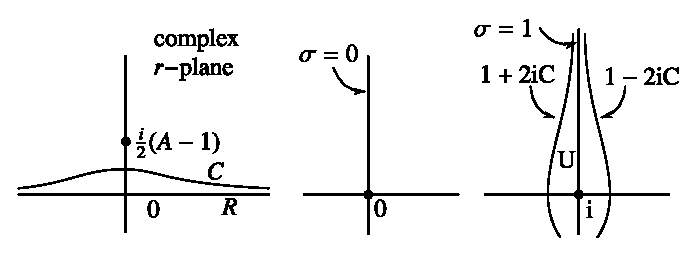
\includegraphics[scale=.85]{chap11/fig1.eps}
\end{figure}
\noindent
$r \in C$ (see figure). The integral $J_C (s)$ converges for all $s \in C$ such that $\zeta^\ast(s + 2 ir)$ and $\zeta^\ast (s - 2 ir)$ remain finite for all $r \in C$, \ie for $s \not\in 1 \pm 2 i C$, $\pm 2 i C$. In particular, $J_C (s)$ is holomorphic in the region $U$ bounded by $1+ 2 i C$ and $1 - 2 i C$. Clearly $J_C (s) = J(s)$ for $s$ to the right of $1 - 2i C$, but for $s$ in the right half of $U$ we have 
$$
J(s) - J_C (s) = \pi \frac{\zeta^\ast (2 s- 1)}{\zeta^\ast (2 -s ) \zeta^\ast (s)} h\left(i\frac{s-1}{2} \right) \quad (s \in U, \re (s) >1)
$$
because the integrand has a simple pole (at $r = \dfrac{1}{2} (s-1)$) with residue $\dfrac{1}{2i} \dfrac{\zeta^\ast (2s-1)}{\zeta^\ast (2 -s) \zeta^\ast (s)} h(\dfrac{i}{2} (s-1))$ in the region enclosed by $\bR$ and $C$. Similarly 
$$
J(s) - J_C (s)= - \pi \frac{\zeta^\ast (2s -1)}{\zeta^\ast (2 -s) \zeta^\ast (s)} h \left(i \frac{s-1}{2} \right) (s \in U , \re (s) < 1).
$$
Therefore the function $J(s)$ in $0 < \sigma < 1$ is $2 \pi \dfrac{\zeta^\ast (2s -1)}{\zeta^\ast (2 -s) \zeta^\ast (s)} h \left(i\frac{s-1}{2} \right)$ less than the analytic continuation of the function defined by $J(s)$ for $\sigma>1$. Together with \eqref{art11-eq3.4} this shows that $I^\ast_4 (s) = \zeta^\ast (2s) I_4 (s)$ has an analytic continuation to $\sigma >0$ given by 
\begin{equation*}
I^\ast_4 (s) = 
\left\{ 
\begin{aligned}
& - \frac{1}{4 \pi} \zeta^\ast (s)^2 J (s)\\[3pt]
& - \frac{1}{4 \pi} \zeta^\ast (s)^2 J_C (s) - \frac{1}{4} \frac{\zeta^\ast (s) \zeta^\ast (2s -1)}{\zeta^\ast (s-1)} h \left(i \frac{s-1}{2} \right) \quad (s \in U), \\[3pt]
& - \frac{1}{4\pi} \zeta^\ast (s)^2 J(s) - \frac{1}{2} \frac{\zeta^\ast (s) \zeta^\ast (2s -1)}{\zeta^\ast (s-1)} h (i\frac{s-1}{2}) \; (0 < \sigma < 1),
\end{aligned} 
\right.
\tag{4.8}\label{art11-eq4.8}
\end{equation*}\pageoriginale
where we have used the functional equation $\zeta^\ast (s) =\zeta^\ast (1-s)$. Of course, we could use a similar argument to extend past the critical line $\sigma =0$, but since it is obvious that $J(s) = J(1-s)$, we deduce from \eqref{art11-eq4.8} that $I^\ast _4(s)$ satisfies the functional equation 
\begin{align*}
I^\ast_4 (1-s) =I^{\ast}_4 (s) & -\frac{1}{2} \frac{\zeta^\ast (s) \zeta^\ast (2s -1)}{\zeta^{\ast} (s-1)} h \left(i \frac{s-1}{2} \right)\\
& + \frac{1}{2} \frac{\zeta^\ast (s) \zeta^\ast (2s)}{\zeta^\ast (s+1)} h \left(i\frac{s}{2} \right),
\end{align*}
and this gives the meromorphic continuation immediately. From \eqref{art11-eq4.8} and \eqref{art11-eq3.5} we find 
\begin{align*}
&I^\ast_3 (s) + I^\ast_4 (s) = -\frac{1}{4 \pi} \zeta^\ast (s)^2 J(s) \tag{4.9}\label{art11-eq4.9}\\
& -\left\{
\begin{aligned}
& \frac{1}{2} \frac{\zeta^\ast (s) \zeta^\ast (2s)}{\zeta^\ast (s+1)} h \left(\frac{is}{2} \right) \quad (1<\sigma <A)\\
& \frac{1}{2} \frac{\zeta^\ast (s) \zeta^\ast (2s)}{\zeta^\ast (s+1)} h \left(\frac{is}{2} \right) + \frac{1}{2} \frac{\zeta^\ast (s) \zeta^\ast (2s-1)}{\zeta^\ast (s-1)} h \left(i \frac{s-1}{2} \right) \; \; (0 < \sigma < 1)\\
& \frac{1}{2} \frac{\zeta^\ast (s) \zeta^\ast (2s -1)}{ \zeta^\ast (s-1)} h \left(i \frac{s-1}{2} \right) \quad (1 - A < \sigma <0),
\end{aligned}
\right.
\end{align*}
which proves the invariance of \eqref{art11-eq4.3} under $s \to 1 -s$. Notice that the function $\sfrac{\zeta^\ast (s) \zeta^\ast (2s)}{\zeta^{\ast} (s+1)}h \left(\dfrac{is}{2} \right) \left(\resp \dfrac{\zeta^\ast (s) \zeta^\ast (2s -1)}{\zeta^\ast (s-1)} h \left(i -\frac{s-1}{2} \right) \right)$  has infini\-tely many\pageoriginale poles in the half-plane $\sigma < 0$ (\resp $\sigma >1$), but drops out of \eqref{art11-eq4.9} before that half-plane is reached. In fact, it is clear from \eqref{art11-eq4.8} and \eqref{art11-eq4.9} that the function $I^\ast_3 (s) + I^\ast_4 (s)$ is holomorphic in $1 - A < \sigma < A$ except for double poles at $s =0$ and $s =1$ (the simple poles at $s = \dfrac{1}{2}$ must cancel since $I^\ast_3(s) + I^\ast_4(s)$ is an even function of $s - \dfrac{1}{2}$).

It remains to treat the function \eqref{art11-eq4.2}. Using the formulas \eqref{art11-eq2.23} for the Selberg transform we find 
\begin{align*}
\int\limits^\infty_0 \varphi (u^2) u^{s-1} du & = - \frac{1}{u} \int\limits^\infty_{0} \int\limits^\infty_{-\infty} Q' (u^2 + v^2) u^{s-1} dv \; du\\
& = -\frac{1}{\pi} \int\limits^\infty_{0} \int\limits^\pi_0 Q'(r^2) (r \sin \theta)^{s-1}  r \; dr d \theta (\re^{i\theta} = v + iu)\\
& = - \frac{\Gamma \left(\frac{s}{2} \right)}{\Gamma (\frac{1}{2}) \Gamma \left(\frac{s+1}{2} \right)} \int\limits^\infty_0 Q' (r^2) r^s dr\\
& = - \frac{\Gamma \left(\frac{s}{2} \right)}{2 \Gamma \left(\frac{1}{2} \right) \Gamma \left(\frac{s+1}{2} \right)} \int\limits^\infty_0 (2 \sinh \frac{u}{2})^{s-1} g' (u) du 
\end{align*}
and hence, by \eqref{art11-eq4.7},
\begin{align*}
& \pi^{-s} \Gamma (s) \zeta (s,0) [V(s,2) + V(s, -2)] =\\
& = - \frac{(4\pi)^{\frac{1}{2} (s-1)}}{\Gamma \left(\frac{s+1}{2} \right)} \zeta^\ast (s) \zeta^\ast(2s -1) \int\limits^\infty_0 \left(\sinh \frac{u}{2} \right)^{s-1} g' (u) du;
\end{align*}
the integral converges for $-1 <\sigma < 1 + A$ and hence gives the analytic continuation of the left-hand side to this strip. On the other hand, formulas \eqref{art11-eq3.7} and \eqref{art11-eq3.8} give
$$
I^\ast_2 (s) = - \frac{(4 \pi)^{-\frac{1}{2}s}}{\Gamma ( 1- \frac{s}{2})} \zeta^\ast (s) \zeta^\ast (2s) \int\limits^\infty_0 (\sinh \frac{u}{2})^{-s} g' (u) du, 
$$\pageoriginale 
where now the integral converges for $-A < \sigma < 2$. This shows that the function \eqref{art11-eq4.2} can be continued to the strip $-A <\sigma < 1+ A$ and is invariant under $s \to 1 -s$; equation \eqref{art11-eq3.9} then gives the formula
\begin{gather*}
\pi^{-s} \Gamma (s) \zeta (s,0) [V (s,2) + V (s,-2)] = I^\ast_2 (1-s) \tag{4.10}\label{art11-eq4.10}\\
= \frac{\zeta^\ast (s) \zeta^\ast (2s -1)}{(4 \pi)^{\frac{2-s}{2}} \Gamma \left(\frac{2-s}{2} \right)} \int\limits^\infty_{-\infty} \frac{\Gamma \left(\frac{1-s}{2} + ir \right) \Gamma \left(\frac{1-s}{2} - ir \right)}{\Gamma (ir) \quad \Gamma (-ir)} h (r) dr \; (0< \sigma <1)
\end{gather*}
in the critical strip. A similar discussion to that given for the integral $I^\ast_4(s)$ now shows that for $\sigma >1$ we must add $\dfrac{\pi^{\frac{1}{2}(s-1)}}{\Gamma \left(\frac{s-1}{2} \right)} \zeta^\ast (s) \zeta^\ast (2s -1) h\left(i \frac{s-1}{2} \right)$ to the right-hand side of \eqref{art11-eq4.10} and that near the line $\sigma =1$ we have 
\begin{gather*}
\pi^{-s} \Gamma (s) \zeta (s,0) [V (s,2) + V(s,-2)]\\
= \frac{\zeta^\ast (s)\zeta^\ast (2s -1)}{(4 \pi)^{\frac{2-s}{2}} \Gamma \left(\frac{2-s}{2} \right) } \int\limits_C \frac{\Gamma \left(\frac{1-s}{2} + ir \right) \Gamma \left(\frac{1-s}{2}  - ir\right)}{\Gamma(ir) \Gamma (-ir)} h (r) dr \tag{4.11}\label{art11-eq4.11}\\
+ \frac{1}{2} \frac{\pi^{\frac{s-1}{2}}}{\Gamma \left(\frac{s-1}{2} \right)} \zeta^\ast (s) \zeta^\ast (2s -1) h (i \frac{s-1}{2}) \quad (s \in U).
\end{gather*}

Again the analytic continuation to $1 - A < \sigma \leqslant 0$ follows using the functional equation.

We have thus proved the analytic continuability and functional equation of each of the functions \eqref{art11-eq4.1} - \eqref{art11-eq4.3} in the strip $1 - A < \sigma < A$ and given\pageoriginale explicit formulas for these functions in each of the five regions $1 - A < \sigma < 0$, $1 - U$, $0< \sigma < 1$, $U$ and $1 <\sigma < A$ covering this strip. We and this section by using these formulas to compute the residue at $s =1$ of the functions in question. 

From the development
$$
\zeta^{\ast} (s) = \frac{1}{s-1} + \frac{1}{2} (\gamma - \log 4 \pi)  + O(s-1) \quad (s\to 1)
$$
and \eqref{art11-eq4.8} we find 
\begin{align*}
I^\ast_4 (s) & = - \frac{1}{4 \pi} \left[\frac{1}{(s-1)^2} + \frac{\gamma - \log 4 \pi}{s -1} + O(1)\right]\\
& \quad \times \left[\int\limits_C h(r) dr + (s-1) \int\limits_C z(r) h(r) dr + O(s-1)^2 \right]\\
& \quad\quad  + \frac{1}{8}  h(0) \frac{1}{s-1} + O(1)
\end{align*}
as $s \to 1$, where $z(r) = \dfrac{zeta^{\ast'} (1+2 ir)}{\zeta^\ast (1+ 2ir )} + \dfrac{\zeta^{\ast'} (1-2ir)}{\zeta^\ast (1-2 ir)}$. Since $z(r)$ is holomorphic for $r$ near the real line (the poles of the two terms at $r=0$ cancel), we can replace $C$ by $\bR$ in the two integrals, obtaining 
\begin{align*}
I^\ast_4 (s) & =  -\frac{\kappa}{(s-1)^2} + \left(-\kappa (\gamma - \log 4 \pi) + \frac{h(0)}{8}  \right.\\
&\left.  - \frac{1}{4 \pi} \int\limits^\infty_{-\infty} z(r) h (r) dr \right) (s-1)^{-1} + O(1)
\end{align*}
as $s \to 1$, where $\kappa = \dfrac{1}{4 \pi} \int\limits^\infty_{-\infty} h(r) dr$. From \eqref{art11-eq3.5} we get 
$$
I^\ast_3 (s) = - \frac{\zeta^\ast (s) \zeta^{\ast} (2s)}{2 \zeta^\ast (s+1)} h \left(\frac{is}{2} \right) = - \frac{1}{2} \frac{h(\frac{i}{2})}{s-1} + O(1) \quad (s \to 1).
$$
This takes care of the function \eqref{art11-eq4.3}. For \eqref{art11-eq4.2} we use equations \eqref{art11-eq4.11} and \eqref{art11-eq3.9},\pageoriginale obtaining (by an argument similar to the one just used for $I^\ast_4$) 
\begin{align*}
& \pi^{-s} \Gamma (s) \zeta(s,0) [V(s,2) + V (s-2)]\\
& = \left[ \frac{1}{s-1} + \frac{1}{2} (\gamma -\log 4 \pi) + O(s-1) \right]\\
&\quad \times \left[\frac{1}{2 (s-1)} + \frac{1}{2} (\gamma - \log 4 \pi) + O(s-1) \right]\\
&\quad \times \left[\frac{1}{2\pi} + \frac{1}{4 \pi} \left(\log 4 \pi +\frac{\Gamma'}{\Gamma} (\frac{1}{2}) \right) (s-1) + O(s-1)^2\right]\\
&\quad \times \left[\int\limits_C h (r)dr - \frac{s-1}{2} \int\limits_C \left(\frac{\Gamma'}{\Gamma} (ir) + \frac{\Gamma'}{\Gamma} (-ir) \right)  h (r) dr \right.\\
&\left.  + O(s-1)^2\right] + \frac{h(0)}{8} (s-1)^{-1} + O(1)\\
& = \frac{\kappa}{(s-1)^2} + \left(\kappa (\gamma - \log 8 \pi) \right.\\
&\left. -\frac{1}{4\pi} \int\limits^\infty_{-\infty} \frac{\Gamma'}{\Gamma} (1 + ir) h (r) dr + \frac{1}{8} h (0) \right) (s-1)^{-1} + O(1)
\end{align*}
and 
$$
I^\ast_2(s) = \left(\frac{1}{24} \int\limits^\infty_{-\infty} h(r) r \tanh \pi r dr \right) (s-1)^{-1} + O(1). 
$$
Finally, to compute the residue of \eqref{art11-eq4.1} at $s=1$ we need the values of $V(1,t)$ and $\res_{s=1} \zeta(s,t^2 -4)$ for $t \in \bZ$, $t \neq \pm 2$. From \eqref{art11-eq4.4} and \eqref{art11-eq4.5} we find 
$$
V(1,t) =
\left\{ 
\begin{aligned}
& \frac{\pi}{2} \int\limits^\infty_0 \varphi (x) \frac{dx}{\sqrt{x+ 4 -t^2}} \quad (|t|<2)\\
& \frac{\pi}{2} \int\limits^\infty_{t^2 -4} \varphi (x) \frac{dx}{ \sqrt{x + 4 -t^2}} \quad (|t|>2)
\end{aligned}
\right.
$$
(since\pageoriginale $P_0 (u) =1$, $F(0, b; c; x) =1$). Using the formulas \eqref{art11-eq2.23} for the Selberg transform, we can express this in therms of $h(r)$, obtaining 
\begin{equation*}
V(1,t) = 
\left\{ 
\begin{aligned}
& \frac{1}{2} \int\limits^\infty_{-\infty} \frac{e^{-2 \alpha r}}{1+e^{-2\pi r}}  h(r)dr \; \left(|t| = 2 \cos \alpha \leqslant 2, \; 0\leqslant \alpha \leqslant \frac{\pi}{2}\right)\\
& \frac{1}{4} \int\limits^\infty_{-\infty} e^{2 i \alpha r} h(r) dr \quad (|t| = 2 \cosh \alpha \geqslant 2)
\end{aligned}
\right.
\tag{4.12}\label{art11-eq4.12}
\end{equation*}
(we omit the calculation, which is not difficult, since in $\S 5$ we will give a general formula for $V (s,t)$ in terms of $h(r)$). As to $\zeta (s,D)$, we have 
\begin{equation*}
\res_{s =1} \zeta (s, D) =
\left\{
\begin{aligned}
\frac{2\pi}{\sqrt{|D|}} \sum\limits_Q \frac{1}{|\Aut (Q)|} \qquad (D<0)\\
\frac{1}{\sqrt{D}} \sum\limits_Q \log \varepsilon_Q \qquad (D > 0), 
\end{aligned}
\right.\tag{4.13}\label{art11-eq4.13}
\end{equation*}
where $\sum\limits_Q$ and $\Aut (Q)$ have the same meaning as in \eqref{art11-eq1.12} and, in the second formula, $\varepsilon_Q$ is the fundamental unit for $Q$ (\ie the larger eigenvalue of $M$, where $M \in SL_2 (\bZ)$ is a matrix with positive trace such that $\Aut (Q) = \{\pm M^n, n \in \bZ\}$).

We have thus given the principal part of each of the functions \eqref{art11-eq4.1}  - \eqref{art11-eq4.3} at the pole $s =1$. Adding up the expressions obtained, we find that the terms in $(s-1)^{-2}$ cancel and that 
\begin{align*}
\sum\limits^\infty_{j=0} h(r_j) & = \int\limits_{\Gamma / \sfH} \left[K_0 (z,z) + \frac{3}{\pi} h\left(\frac{i}{2} \right) \right] dz = 2 \res_{s=1} I^\ast (s) + h \left(\frac{i}{2} \right)\\
& =\frac{1}{12} \int\limits^\infty_{-\infty} h(r) r \tanh \pi r dr\tag{4.14}\label{art11-eq4.14}\\
& \qquad - \frac{1}{2 \pi } \int\limits^\infty_{-\infty} \left(z(r) + \frac{\Gamma'}{\Gamma} (1+ ir) + \log 2 \right) h (r) dr\\
& + \frac{1}{2} h(0) + \frac{2}{\pi} \sum\limits^\infty_{\substack{t = - \infty\\ t^2 \neq4}} V(1,t) \res_{s=1} \zeta (s, t^2 -4),
\end{align*}
where\pageoriginale
\begin{align*}
z(r) &= \frac{\zeta^{\ast'} (1+ 2 ir)}{\zeta^\ast (1+ 2 ir)} + \frac{\zeta^{\ast'} (1-2 ir)}{\zeta^{\ast} (1-2ir)}\\
& = \frac{1}{2} \frac{\Gamma'}{\Gamma} (\frac{1}{2} + ir) - \frac{1}{2} \frac{\Gamma'}{\Gamma} (ir) + \frac{\zeta'}{\zeta} (1+ 2 ir) - \frac{\zeta'}{\zeta} (2 ir)
\end{align*}
and  $V(1,t)$, $\res_{s=1} \zeta (s, t^2 -4)$ are given by equations \eqref{art11-eq4.12} and \eqref{art11-eq4.13}, respectively. Formula \eqref{art11-eq4.14} is the Selberg trace formula.

\S~5. \text{Complements.} In the last section we gave the analytic continuation of $I(s)$ to the strip $1- A <\sigma <A$. To complete the proof of Theorem \ref{art11-thm1} we must still
\begin{itemize}
\item[1)] express $V(s,t)$ in terms of the Selberg transform $h(r)$;

\item[2)] generalize the formula obtained for $I(s)$ to the function 
\end{itemize}
\begin{equation*}
I^m (s) =\sum\limits^\infty_{j=1} a_j (m) \frac{h(r_j)}{(f_j, f_j)} R_{f_j} (s) \qquad (m \in \bZ) \tag{5.1}\label{art11-eq5.1}
\end{equation*}
with $m \neq 1$ (notations as in $\S~1$). In this section we will carry out these two calculations and also indicate the generalization to congruence subgroups of $SL_2 (\bZ)$.

The results of $\S~4$ show that $I^\ast (s)$ equals 
\begin{align*}
& -\frac{1}{4\pi} \zeta^\ast (s)^2 \int\limits^\infty_{-\infty} \frac{\zeta^\ast (s+ 2 ir) \zeta^{\ast} (s -2 ir)}{\zeta^\ast (1+2 ir ) \zeta^\ast (1 - 2 ir)} h (r) dr\\ 
& - \frac{1}{2} \frac{\zeta^\ast (s) \zeta^\ast (2s)}{\zeta^\ast (s+1)} h \left(\frac{is}{2} \right) - \frac{1}{2} \frac{\zeta^\ast (s) \zeta^\ast (2s-1)}{\zeta^\ast (s-1)} h \left(i \frac{1-s}{2} \right)\\
& + \frac{\zeta^\ast (s) \zeta^\ast (2s)}{(4 \pi)^{\frac{s+1}{2}} \Gamma \left(\frac{s+1}{2} \right)} \int\limits^{\infty}_{-\infty} \frac{\Gamma \left(\frac{s}{2} + ir \right) \Gamma \left(\frac{s}{2} - ir \right)}{\Gamma (ir) \Gamma (-ir)} h (r) dr\\
& = \frac{\zeta^\ast (s) \zeta^\ast (2s -1)}{(4 \pi)^{\frac{2-s}{2}} \Gamma\left(\frac{2-s}{2} \right)} \int\limits^\infty_{-\infty} \frac{\Gamma \left(\frac{1-s}{2} + ir \right) \Gamma \left(\frac{1-s}{2} -ir \right)}{ \Gamma (ir) \Gamma (-ir)} h (r) dr \\
& + \pi^{-s} \Gamma (s) \sum\limits^\infty_{\substack{t = -\infty\\ t^2\neq 4}} V (s,t) \zeta (s, t^2 -4)
\end{align*}\pageoriginale
in the critical strip $0<\sigma<1$ (cf. equations \eqref{art11-eq4.9} and \eqref{art11-eq4.10}. Using the functional equations of $V(s,t)$ and $\zeta(s,D)$ we can write this expression as $\mathscr{R}(s)+\mathscr{R}(l-s)$, where
\begin{align*}
\mathscr{R}(s) &= -\dfrac{1}{8\pi}\zeta^{*}(s)^{2} \int\limits^{\infty}_{-\infty}\dfrac{\zeta^{*}(s+2ir)\zeta^{*}(s-2ir)}{\zeta^{*}(1+2ir)\zeta^{*}(1-2ir)}h(r)dr\\
&\quad -\dfrac{\zeta^{*}(s)\zeta^{*}(2s)}{2\zeta^{*}(s+1)}h\left(\dfrac{is}{2}\right)\\
&\quad +\dfrac{\Gamma(s)\Gamma(s-\frac{1}{2})}{2\pi^{s}\Gamma\left(\frac{2-s}{2}\right)\Gamma\left(\frac{1+s}{2}\right)}\zeta(s)\zeta(2s-1)\times\\
&\quad \int\limits^{\infty}_{-\infty}\dfrac{\Gamma\left(\frac{1-s}{2}+ir\right)\Gamma\left(\frac{1-s}{2}-ir\right)}{\Gamma(ir)\Gamma(-ir)}h(r)dr\\
&\quad +\pi^{-s}\Gamma(s)\sum\limits^{\infty}_{\substack{t=-\infty\\ t\neq \pm 2}}v(s,t)\zeta(s,t^{2}-4),
\end{align*}
$v(s,t)$ being any function such that 
\begin{equation*}
V(s,t) = v(s,t) + \frac{\pi^{s-1} \Gamma (1-s)}{\pi^{-s} \Gamma (s)} \frac{\Gamma (s, \Delta)}{\gamma (1-s, \Delta)} v (1-s,t). 
\tag{5.2}\label{art11-eq5.2}
\end{equation*}
(here $\Delta = t^2 -4$ as before). Comparing this with \eqref{art11-eq1.16} and observing that $F(a,b; c;0) =1$, we see that Theorem \ref{art11-thm1} (for $m=1$) will follow from
\end{proof}

\medskip
\noindent
{\bfseries Proposition \thnum{5}:\label{art11-prop5}}
For $t \neq \pm 2$ and $0 < \re (s) < 1$ the function $V(s,t)$ defined by \eqref{art11-eq3.10}\pageoriginale  is given by equation \eqref{art11-eq5.2} with 
\begin{align*}
v(s,t)& =\frac{\Gamma(s - \frac{1}{2})}{4 \Gamma \left(\frac{s+1}{2}  \Gamma \left(\frac{2-s}{2} \right)\right)} \int\limits^\infty_{-\infty} \frac{\Gamma \left(\frac{1-s}{2} + ir \right) \Gamma \left(\frac{1-s}{2} - ir \right)}{\Gamma (ir) \Gamma (-ir)}\\
&\quad \times F \left(\frac{1-s}{2} + ir, \frac{1-s}{2} - ir; \frac{3}{2} -s ; 1 - \frac{t^2}{4} \right) h(r) dr. 
\end{align*} 

\begin{proof}
As in Proposition \eqref{art11-prop4} we must distinguish the cases $\Delta > 0$ and $\Delta < 0$. It will also be useful  to introduce symmetrization operators $\sS^1_s, \sS_r$ with 
$$
\sS^1_s [f(s)] = f(s) + f (1-s), \quad \sS_r [f(s)] = f(r) + f (-r)
$$
for any function $f$. Thus the formula we want to prove can be written 
\begin{equation*}
\frac{\pi^{-s} \Gamma (s)}{\Gamma (s, \Delta)} V (s,t) = \sS^1_s \left[\frac{\pi^{-s} \Gamma (s)}{\gamma (s, \Delta)} v (s,t) \right].
\tag{5.3}\label{art11-eq5.3}
\end{equation*}
If $\Delta >0$, then \eqref{art11-eq4.5} and \eqref{art11-eq2.24} give 
\begin{align*}
V(s,t) & =\frac{1}{8\pi} \frac{\Gamma \left(\frac{s}{2} \right)}{\Gamma (s)} \Delta^{\frac{s}{2}} \int\limits^\infty_{-\infty} r \tanh \pi r h (r)\\
& =\times \int\limits^1_0 O\P_{-\frac{1}{2} + ir} \left(1+ \frac{\Delta/ 2}{1-\xi} \right) (1-\xi)^{\frac{s-3}{2}} F \left(\frac{s}{2}, \frac{s}{2}; \frac{1}{2} ; \xi \right) \frac{d\xi}{\sqrt{\xi}} dr, 
\end{align*}
where we have made the change of variables $\xi =\dfrac{u^2}{u^2+1}$. To prove \eqref{art11-eq5.3}, we must show that the inner integral equals 
\begin{align*}
& \sS^1_s \left[\frac{2^s}{\Delta^{s/2}} \cosh \pi r \frac{\Gamma (S-\frac{1}{2}) \Gamma \left(\frac{1-s}{2} + ir \right) \Gamma \left(\frac{1-s}{2}\right) -ir}{\Gamma \left(\frac{1}{2} \right) \Gamma \left(\frac{s}{2} \right) \Gamma \left(1-\frac{s}{2} \right)} \right.
\tag{5.4}\label{art11-eq5.4}\\
&\quad \left. {}\times F\left(\frac{1-s}{2} + i r, \frac{1-s}{2} - ir ; \frac{3}{2} - s ; 1 - \frac{t^2}{4} \right) \right]
\end{align*}
(here\pageoriginale and from now one we use standard identities for the gamma function without special mention). Using the identity 
{\fontsize{10}{12}\selectfont
$$
P_{-\frac{1}{2} + ir} \left(1+\frac{2}{x} \right) = \sS_r 
\left[ \frac{\Gamma (2 ir)}{\Gamma \left(\frac{1}{2} + ir \right)^2} x^{\frac{1}{2} -ir} F \left(\frac{1}{2}  - ir ,\frac{1}{2}- ir; 1-2 ir; -x \right)\right] (x >0)
$$}\relax
[EH 3.2 (19)] and expanding the hypergeometric series, we find that the integral in question equals 
\begin{multline*}
\sS_r \left[\frac{\text{coth} \pi r}{2 \pi i} \sum\limits^\infty_{n=0} \frac{(-1)^n}{n!} \frac{\Gamma \left(n+ \frac{1}{2} - ir \right)^2}{\Gamma (n+1 - 2 i r)} \left(\frac{\Delta}{4} \right)^{-n -\frac{1}{2} + ir}  \right.\\
\left.  \times \int\limits^1_0 (1-\xi)^{\frac{s}{2} + n -1 - ir} F\left(\frac{s}{2}, \frac{s}{2}; \frac{1}{2}; \xi \right) \frac{d\xi}{\sqrt{\xi}} \right].
\end{multline*}
From [EH 2.4(2), 2.8(46)] we have 
\begin{align*}
& \int\limits^1_0 (1-\xi)^{\frac{s}{2} + n - 1 - ir} \xi^{-\frac{1}{2}} F\left(\frac{s}{2}, \frac{s}{2} ; \frac{1}{2}; \xi  \right) d \xi\\
&\qquad = \frac{\Gamma \left(\frac{1}{2} \right)  \Gamma \left(\frac{s}{2}+ n - ir \right)}{
\Gamma \left(\frac{1+s}{2} + n - ir \right)} F \left(\frac{s}{2} , \frac{s}{2}; \frac{1+s}{2} + n -ir; 1 \right) \\
&\qquad = \frac{\Gamma \left(\frac{s}{2} + n - ir \right) \Gamma \left(\frac{1-s}{2} + n - ir \right) \Gamma \left(\frac{1}{2} \right)}{\Gamma \left(n+ \frac{1}{2} -ir \right)^2},
\end{align*}
so our integral equals 
\begin{align*}
& \sS_r \left[ \frac{\coth \pi r}{2 i \sqrt{\pi}} \sum\limits^\infty_{n=0} \frac{(-1)^n}{n!}  \times  \right.\\
& \qquad \left.\times \frac{\Gamma \left(\frac{s}{2} + n - ir \right)\Gamma \left(\frac{1-s}{2} + n - ir \right)}{\Gamma (n+ 1 - 2 ir)} \left(\frac{\Delta}{4} \right)^{-n -\frac{1}{2} + ir} \right]\\
& = \sS_r \left[ \frac{\coth \pi r }{2i \sqrt{\pi}} \frac{\Gamma \left(\frac{s}{2} - ir \right) \Gamma \left(\frac{1-s}{2} - ir \right)}{\Gamma (1 - 2 ir)} \left(\frac{\Delta}{4} \right)^{ir - \frac{1}{2}}\right. \tag{5.5}\label{art11-eq5.5}\\
&\quad \quad \left.  \times F \left(\frac{s}{2} - ir , \frac{1-s}{2} - ir; 1 - 2 ir ; -\frac{4}{\Delta} \right)\right]\\
& = \sS_r \sS^1_s \left[\frac{\coth \pi r}{ 2 i \sqrt{\pi}} \frac{\Gamma (s - \frac{1}{2}) \Gamma \left(\frac{1-s}{2} -ir \right) }{\Gamma \left(\frac{1+s}{2} - ir \right)} \left(\frac{\Delta}{4} \right)^{-\frac{s}{2}} \right. \\ 
& \left. \times F \left(\frac{1-s}{2} - ir, \frac{1-s}{2} + ir; \frac{3}{2} - s ; -\frac{\Delta}{4} \right)\right]
\end{align*}\pageoriginale
(the last formula is [EH 2.10(2)]), and since 
$$
\sS_r \left[\frac{\coth \pi r}{2 i \sqrt{\pi}} \frac{\Gamma \left(\frac{1-s}{2} -ir \right)}{\Gamma \left(\frac{1+s}{2} -ir\right)} \right] = \frac{\cosh \pi r \Gamma \left(\frac{1-s}{2} + ir \right) \Gamma \left(\frac{1-s}{2} -ir \right)}{ \Gamma \left(\frac{1}{2} \right) \Gamma \left(\frac{s}{2} \right) \Gamma \left(1-\frac{s}{2} \right)}
$$
this agrees with \eqref{art11-eq5.4}, completing the proof for $\Delta > 0$.

If  $\Delta < 0$, then $\dfrac{\pi^{-s} \Gamma (s)}{\gamma (s, \Delta)} = \delta^{-s/2}$, where $\delta = \dfrac{1}{2} |\Delta| = 1 -\dfrac{t^2}{4}$, so \eqref{art11-eq5.3} is equivalent to 
$$
\delta^{-s/2} V (s,t) = \sS^1_s \left[\delta^{\frac{1}{2} (s-1)}  v(1 - s, t)\right].
$$
On the other hand, from \eqref{art11-eq4.4} and \eqref{art11-eq2.24} we have 
$$
\pi^{-s/2} V (s,t) = \frac{1}{2} \int\limits^\infty_{-\infty} r \tanh \pi r h(r) \int\limits^\infty_{1} P_{-\frac{1}{2}+ ir} (1+ 2 \delta (u^2 -1)) P_{-s} (u) du dr. 
$$
Denote\pageoriginale the inner integral by $I$. Then \eqref{art11-eq5.3}  will be proved if we show that 
\begin{align*}
I & = \sS^1_s \left[\frac{1}{2} \delta^{\frac{1}{2} (s-1)}\frac{\Gamma \left(\frac{1}{2} -s \right) \Gamma \left(\frac{s}{2} + ir \right) \Gamma \left(\frac{s}{2} - ir \right)}{\Gamma \left(\frac{1}{2} + ir \right) \Gamma \left(\frac{1}{2}  - ir \right) \Gamma \left(\frac{2-s}{2} \right) \Gamma \left(\frac{1+s}{2} \right)}   \right.\\
& \qquad \left. F \left(\frac{s}{2} + ir , \frac{s}{2} - ir; \frac{1}{2} + s ; \delta \right) \right].
\end{align*}
By [EH 2.10(1)], this is equivalent to 
\begin{gather*}
I = \frac{1}{2 \sqrt{\pi}} \frac{\Gamma \left(\frac{s}{2} + ir \right) \Gamma \left(\frac{s}{2} -ir \right) \Gamma \left(\frac{1-s}{2} + ir \right) \Gamma \left(\frac{1-s}{2} - ir \right)}{\Gamma \left(\frac{1}{2} +ir \right) \Gamma \left(\frac{1}{2} - ir \right) \Gamma \left(\frac{1+s}{2} \right) \Gamma \left(\frac{2-s}{2} \right)}\\
\times \delta^{s-\frac{1}{2}} F \left(\frac{s}{2}  - ir, \frac{s}{2} + ir; \frac{1}{2} ; 1-\delta \right).
\end{gather*}
To prove this this formula, we being by making the substitution $v = u^2 -1$ in $I$ and substituting for $P_{-\frac{1}{2} + ir}$ by 
$$
\int\limits^\infty_0 e^{-ax} K_{ir} (x) \frac{dx}{\sqrt{x}} = \sqrt{\frac{\pi}{2}} \Gamma \left(\frac{1}{2} + ir \right)\Gamma  \left(\frac{1}{2} - ir \right) P_{-\frac{1}{2} + ir} (a)
$$
[GR 6.628. 7]; after an interchange of integration this gives 
\begin{gather*}
\sqrt{2\pi} \Gamma \left(\frac{1}{2} + ir \right) \Gamma \left(\frac{1}{2} -ir \right) I\\
= \int\limits^\infty_0 \left(\int\limits^\infty_0 e^{-2\delta x v} P_{-s} (\sqrt{1+v}) \frac{dv}{\sqrt{1+v}} \right) e^{-x} K_{ir} (x) \frac{dx}{\sqrt{x}}.
\end{gather*}
By [GR 7.146.2] the inner integral equals $(2 \delta x)^{-3/4} e^{\delta x} W_{-\frac{1}{4}, \frac{1}{4} -\frac{s}{2}} (2 \delta x)$, where $W_{\lambda, \mu}$  is Whittaker's function, and using the Mellin-Barnes integral representation of the latter [GR 9.223] we find that this in turn equals 
\begin{gather*}
\Gamma \left(\frac{1+s}{2} \right)^{-1} \Gamma \left(1-\frac{s}{2} \right)^{-1} \cdot \frac{1}{2 \pi i} \int\limits^{C + i \infty}_{C - i \infty} \Gamma \left(v+ \frac{1}{2}\right) \Gamma \left(\frac{s}{2}-v) \Gamma (\frac{1-s}{2} -v\right) \times \\
\times (2\delta x)^{v - \frac{1}{2}} d v, 
\end{gather*}\pageoriginale
where $C$ is chosen such that $-\frac{1}{2} < C < \frac{1}{2} \min (\sigma, 1 -\sigma)$. If choose $C$ to satisfy also $C>0$ then we may interchange the order of integration again, obtaining
\begin{align*}
& 2 \sqrt{\pi} \Gamma \left(\frac{1}{2} + ir\right) \Gamma (\frac{1}{2} -ir) \Gamma \left(\frac{1+s}{2} \right) \Gamma \left(1-\frac{s}{2} \right) I\\
&  =\frac{1}{2 \pi i} \int\limits^{C+ i \infty}_{C -  i \infty} 2^v \delta^{v -\frac{1}{2}} \Gamma (v + \frac{1}{2}) \Gamma \left(\frac{s}{2} -v \right) \Gamma \left(\frac{1-s}{2} - v \right) \times \\
& \qquad \times \int\limits^\infty_{0} x^{v-1} e^{-x} K_{ir} (x) dx \; d v\\
& =\frac{\Gamma (\frac{1}{2})}{2 \pi i} \int\limits^{C + i \infty}_{C - i \infty} \Gamma \left(\frac{s}{2} -v \right) \Gamma \left(\frac{1-s}{2} -v \right) \Gamma (v+ ir) \Gamma (v - ir) \delta^{v -\frac{1}{2}} dv 
\end{align*}
[ET 6.8(28)]. The integral is very rapidly convergent (the integrand is $O(|v|^{-3/2} e^{-2 \pi|v|})$), so we may substitute for $\delta^{v -\frac{1}{2}}$ the binomial expansion
$$
\delta^{v -\frac{1}{2}} =\delta^{\frac{1}{2} (s-1)} \sum\limits^\infty_{n=0} \frac{1}{n!}  \frac{\Gamma \left(\frac{s}{2} - v + n \right)}{\Gamma \left(\frac{s}{2} -v \right)} (1-\delta)^n
$$
and integrate term by term. Using ``Barnes' Lemma''
\begin{gather*}
\frac{1}{2 \pi i} \int\limits^{C + i \infty}_{C - i \infty} \Gamma (\alpha +s) \Gamma (\beta +s) \Gamma (\gamma -s) \Gamma (\delta -s) ds\\
= \frac{\Gamma (\alpha + \gamma) \Gamma (\alpha + \delta) \Gamma (\beta + \gamma) \Gamma (\beta + \delta)}{\Gamma (\alpha + \beta + \gamma + \delta)}
\end{gather*}
[GR 6.412] we obtain finally
\begin{gather*}
2 \Gamma \left(\frac{1}{2} + ir \right) \Gamma \left(\frac{1}{2} - ir \right) \Gamma \left(\frac{1+s}{2} \right) \Gamma \left( 1-\frac{s}{2}\right) I = \delta^{\frac{1}{2} (s-1)} \times \\
\times \sum\limits^\infty_{n=0}  \frac{\Gamma \left(\frac{s}{2} + ir + n \right) \Gamma \left(\frac{s}{2} - ir + n\right) \Gamma \left(\frac{1-s}{2}+ ir \right) \Gamma \left(\frac{1-s}{2} - ir \right)}{\Gamma \left(\frac{1}{2} +n \right) n!} (1-\delta)^n\\
= \Gamma \left(\frac{1}{2}  \right)^{-1} \Gamma \left(\frac{s}{2} +ir \right)  \Gamma \left(\frac{s}{2} - ir \right) \Gamma \left(\frac{1-s}{2} + ir \right) \Gamma \left(\frac{1-s}{2}- ir \right) \delta^{\frac{s-1}{2}}\\
 \times  F \left(\frac{s}{2} + ir , \frac{s}{2} - ir ; \frac{1}{2}; 1 - \delta \right).
\end{gather*}\pageoriginale

This completes the proof of Proposition \ref{art11-prop5} and hence of Theorem \eqref{art11-thm1} for $m=1$. 

To calculate the function \eqref{art11-eq5.1} for $m >1$ we set 
$$
K^m_0 (z,z') = \sum\limits^\infty_{j=1} a_j(m) \frac{h(r_j)}{(f_j, f_j)} f_j (z) \overline{f_j (z')}. 
$$ 
Then $I^m (s) = \int\limits_{\Gamma / \sfH} K^m_0 (z,z) E (z,s)dz$. On the other hand, from \eqref{art11-eq1.6} we see that $K^m_0 (z,z') = m^{\frac{1}{2}} K_0 (z,z') | T (m)$, where $K_0 (z,z')$ is the kernel function \eqref{art11-eq2.27} and $T(m)$ the Hecke operator \eqref{art11-eq1.5}, acting (say) on $z'$. Since the constant function and the Eisenstein series $E(z,s)$ are eigen-functions of $m^{\frac{1}{2}} T(m)$ with eigenvalues $\tau_{\frac{1}{2}} (m)$ and $\tau_{s-\frac{1}{2}} (m)$, respectively ($\tau_v (m)$ as in \eqref{art11-eq2.7}), equation \eqref{art11-eq2.31} gives
\begin{multline*}
K^m_0 (z,z') = K^m (z,z') - \frac{3}{\pi} \tau_{\frac{1}{2}} (m) h \left(\frac{i}{2} \right) -\\
- \frac{1}{4 \pi} \int\limits^\infty_{-\infty} E(z, \frac{1}{2} + ir) E (z' , \frac{1}{2}  - ir) h (r) \tau_{ir} (m) dr, 
\end{multline*}
 where
$$
K^m (z,z') = \sqrt{m} K (z,z') | T (m) = \frac{1}{2\sqrt{m}} \sum\limits_{\substack{a,b,c,d\in\bZ\\ ad - bc =m}} k \left(z, \frac{az' + b}{ cz' + d} \right).
$$
Hence the constant term $\sK^m (y)$ of $K^m_0(z,z)$ equals $\sum\limits^4_{i=1} \sK^m_i (y)$, where $\sK^m_3$ and $\sK^m_4$ are defined exactly like $\sK_3$ and $\sK_4$ but with $h(r)$ replaced  by $h(r) \tau_{ir} (m)$\pageoriginale and
\begin{align*}
\sK^m_1 (y) &= \frac{1}{\sqrt{m}} \int\limits^{iy+1}_{iy} \sum\limits_{\substack{ad- bc=m\\c>0}} k \left(z, \frac{az+b}{cz+d} \right)  dz,\\
\sK^m_2 (y) &= \frac{1}{\sqrt{m}}  \int\limits^{iy+1}_{iy} \sum\limits_{\substack{ad = m\\a,d>0}} \sum\limits^\infty_{b=-\infty} k \left(z, \frac{az+b}{d} \right) dz - \\
&  \quad  - \frac{y}{2 \pi} \int\limits^\infty_{-\infty} h(r) \tau_{ir} (m) dr. 
\end{align*}
As in \S 3 we then find $I^m(s) = \sum\limits^4_{i=1} I^m_i (s)$ for $1<\sigma <A$, where $I^m_3$ and $I^m_4$ are given by the same formulas as $I_3$ and $I_4$ (equations \eqref{art11-eq3.4} and \eqref{art11-eq3.5}) but with $h(r)$ replaced by $\tau_{ir} (m) h(r)$ and 
$$
\zeta(2s) I^m_1 (s) = m^{\frac{s-1}{2}} \sum\limits^\infty_{t = - \infty} \zeta (s, t^2 - 4 m) V \left(s, \frac{t}{\sqrt{m}}\right).
$$
As to $I^m_2$, from \eqref{art11-eq2.20} and \eqref{art11-eq2.23} we find 
\begin{align*}
\sK^m_2 (y) & = \frac{1}{\sqrt{m}} \int\limits^1_0 \sum\limits_{\substack{ad=m\\ a, d>0}} \sum\limits^\infty_{b = - \infty} \varphi \left(\frac{(x (d-a) -b)^2 + (a-d)^2 y^2}{my^2} \right) dx \\
& - \qquad \frac{y}{2\pi} \sum\limits_{\substack{ad =m\\ a, d>0}} \int\limits^\infty_{-\infty} h(r) \left(\frac{a}{d} \right)^{ir} dr \\
& = \frac{1}{\sqrt{m}} \sum\limits_{\substack{ad = m\\ a\neq d}} Q \left(\frac{(a-d)^2}{m} \right) -y \sum\limits_{ad = m} g \left(\log \frac{a}{d} \right)\\
& + 
\left\{
\begin{aligned}
\frac{1}{\sqrt{m}} \sum\limits^\infty_{b = - \infty} \varphi \left(\frac{b^2}{my^2} \right) &\quad \text{ if } \sqrt{m} \in \bZ\\
0& \quad \text{ if }\sqrt{m} \not\in \bZ
\end{aligned}
\right.\\
& = 
\left\{
\begin{aligned}
\frac{1}{\sqrt{m}} \sK_2 (y \sqrt{m}) & \quad  \text{ if } \sqrt{m} \in \bZ\\
0 & \quad \text{ if } \sqrt{m} \not\in \bZ,
\end{aligned}
\right.
\end{align*}
so\pageoriginale 
$$
I^m_2 (s) = 
\left\{ 
\begin{aligned}
m^{-s/2} I_2 (s) & \quad \text{ if } \sqrt{m} \in \bZ,\\
0 & \quad \text{ if } \sqrt{m} \not\in \bZ.
\end{aligned}
\right.
$$
The analytic continuation to $1 - A < \sigma <1 $ now proceeds as in \S~4, the only essential difference being that the terms \eqref{art11-eq4.2} are absent when $m$ is not a square, since $I^m_1$ then has no summands with $t^2 - 4 m = 0$ and $I^m_2$ vanishes identically. The final formula is that given in Theorem \ref{art11-thm1}.

If $m < 0$ the proof is similar and in fact somewhat easier (since $t^2- 4 m$ now always has the same sign and the term $I_2$ is absent), but the calculations with the hypergeometric functions are a little different. Since constant functions and Eisenstein series are invariant under $T(-1)$, the terms $I^m_3 (s)$ and $I^m_4(s)$ are equal to $I^{|m|}_3(s)$ and $I^{|m|}_4(s)$, so that first two terms in \eqref{art11-eq1.16} are unchanged except for replacing $m$ by $|m|$. The term $I^m_2$ is always zero since $m$ cannot be a square. Finally, for $I^m_1$ we find 
\begin{equation*}
I^m_1 (s) = |m|^{\frac{s-1}{2}} \sum\limits^\infty_{t = - \infty} \frac{\zeta(s,t^2 - 4 m)}{\zeta(2s)} V_{s, t |m|^{-\frac{1}{2}}} \quad (m<0)\tag{5.6}
\label{art11-eq5.6}
\end{equation*}
with
$$
V_{s,t} = \int\limits_{\sfH} k \left(z, \frac{1}{\bar{z} + t} \right) y^s dz = \int\limits_{\sfH} \varphi \left(\frac{\left(|z|^2 - \Delta / 4 \right)^2}{y^2} + t^2 \right) y^s dz,
$$
where now $\Delta = t^ +4$. This function is easier to compute than $V(s,t)$ since $\Delta$ always has the same sign. Making the same substitutions as in the case $\Delta >0$ of Proposition \eqref{art11-prop4} we find that $V_-(s,t)$ is given by the same integral \eqref{art11-eq4.5} but with $\varphi (\Delta u^2 + t^2)$ instead of $\varphi (\Delta u^2+ \Delta)$, This integral can then be calculated as in the case $\Delta > 0$ of Proposition \ref{art11-prop5}, the only difference being that the function $P_{-\frac{1}{2} + ir} \left(1+\dfrac{\Delta /2}{1-\xi} \right)$ is replaced by $P_{-\frac{1}{2} + ir} \left(-1 + \dfrac{\Delta /2}{1-\xi}\right)$ and we must use
\begin{multline*}
P_{-\frac{1}{2} + ir} \left(-1 + \frac{2}{x}  \right) =  \\
 = \sS_r \left[ \frac{\Gamma (2 ir)}{\Gamma \left(\frac{1}{2} + ir \right)^2} x^{\frac{1}{2} - ir} F \left(\frac{1}{2}  - ir, \frac{1}{2} - ir; 1 - 2 ir; x \right) \right] \;\; (x>0)
\end{multline*}\pageoriginale
[EH 3.2(18)] instead of the corresponding formula for $P_{-\frac{1}{2} + ir} \left(1+ \dfrac{2}{x} \right)$. This has the effect of introducing an extra factor $(-1)^n$ in the infinite sum and hence of replacing the argument $-\dfrac{4}{\Delta}$ in \eqref{art11-eq5.4} by $+ \dfrac{4}{\Delta}$. Using the identity 
\begin{gather*}
\sS_r \left[\frac{\coth \pi r}{2i \sqrt{\pi}}  \frac{\Gamma \left(\frac{s}{2} - ir \right) \Gamma \left(\frac{1-s}{2} - ir \right)}{\Gamma (1 - 2 ir)} \left(\frac{\Delta}{4} \right)^{ir - \frac{1}{2}} \times \right.\\
\left. \times F \left(\frac{s}{2}  - ir, \frac{1-s}{2} - ir; 1 - 2 ir; \frac{4}{\Delta} \right)  \right]\\
=\frac{\cosh^2 \pi r}{\pi^2} \Gamma \left(\frac{s}{2} + ir \right) \Gamma \left(\frac{s}{2}  - ir \right) \Gamma\left(\frac{1-s}{2} + ir  \right) \Gamma \left(\frac{1-s}{2} -ir \right) \left(\frac{\Delta}{4} \right)^{-\frac{s}{2}}. \times \\
\times F \left( \frac{1-s}{2} - ir, \frac{1-s}{2} +ir; \frac{1}{2} ; 1 -\frac{\Delta}{4}\right)
\end{gather*}
[EH 2.10(3)] and substituting the expression thus obtained for $V_-(s,t)$ into \eqref{art11-eq5.6}, we find that the last term in \eqref{art11-eq1.16} must be replaced by
\begin{gather*}
\frac{2^{s-4}  |m|^{\frac{s-1}{2}}}{\pi^{s+1}} \Gamma \left(\frac{s}{2} \right)^2 \sum\limits^\infty_{t = - \infty} \zeta (s, t^2 - 4 m) \times \\
\times \int\limits^\infty_{-\infty} \frac{\Gamma \left(\frac{s}{2} + ir \right) \Gamma \left(\frac{s}{2} - ir \right) \Gamma \left(\frac{1-s}{2} + ir \right) \Gamma \left(\frac{1-2}{2} - ir \right)}{\Gamma \left(\frac{1}{2} + ir \right) \Gamma\left(\frac{1}{2} - ir \right) \Gamma (ir) \Gamma (-ir)} \\
\times F \left(\frac{1-s}{2} + ir, \frac{1-s}{2} - ir ; \frac{1}{2} ; \frac{t^2}{4 m} \right) h (r) dr
\end{gather*}
if $m <0$. This completes the proof of Theorem \eqref{art11-thm1}.

Finally,\pageoriginale we indicate what happens when $\Gamma$ is replaced by a congruence subgroup $\Gamma_1$ in the simplest case $\Gamma_1 = \Gamma_0 (q) / \{ \pm 1\}$, $q$ prime. There are now two cusps and correspondingly two Eisenstein series $E_1$ and $E_2$, given explicitly by 
$$
E_1 (z) = \sum\limits_{\gamma \in \Gamma_\infty \backslash \Gamma_1} \Iim (\gamma z)^s, \quad E_2 (z) = \sum\limits_{\gamma \in w^{-1} \Gamma_\infty w \backslash \Gamma_1} \Iim (w \gamma z)^s
$$
(where $w = \left(\begin{matrix}
0 & -1\\q & 0
\end{matrix}
\right)$), and formula \eqref{art11-eq2.31} becomes 
\begin{gather*}
K_0 (z,z') =\sum\limits_{\gamma \in \Gamma_1} k(z, \gamma z') -\frac{1}{\vol (\Gamma_1 \backslash \sfH)} h \left(\frac{i}{2} \right)-\\
- \frac{1}{4\pi} \sum\limits^2_{j=1} \int\limits^\infty_{-\infty} E_j (z, \frac{1}{2} + ir) E_j (z' , \frac{1}{2} - ir) h(r) dr, 
\end{gather*}
where $K_0 (z,z')$ is defined as before but with $f_j$ now running over all Maass cusp forms of weight 0 on $\Gamma_1$ (\cf \cite{art11-4}). It is easily checked that 
\begin{align*}
E_1 (z,s) & = \frac{q^s}{q^{2s}-1} E (qz, s) - \frac{1}{q^{2s} -1} E (z,s),\\
E_2 (z,s) & = \frac{q^s}{q^{2s} -1} E(z,s) - \frac{1}{q^{2s} -1} E(qz,s),
\end{align*}
 so that Fourier developments of $E_1$ and $E_2$ can be deduced from \eqref{art11-eq2.6}. The calculation of $I(s) = \int\limits_{\Gamma_1 / \sfH} K_0 (z,z) E_1 (z,s) dz$ (which again can be expressed as $\int\limits^\infty_0 \sK (y) y^{s-2} dy$, $\sK (y)$ = constant term of $K_0 (z,z)$) now proceeds as in \S~3; the final formula is the same except that $I_1 (s)$ is replaced by
$$
\frac{1}{q^2 +1} \zeta(2s)^{-1} \sum\limits^\infty_{t = - \infty} \left(1+ \left(\frac{t^2 - 4}{q} \right) \right) \zeta(s, t^2 - 4) V (s,t),
$$ 
(where $\left(\dfrac{\Delta}{q} \right)$ is the Legendre symbol), $I_3 (s)$ is multiplied by $\dfrac{q-1}{q^{s+1} -1}$, and the integrand of $I_4 (s)$ is multiplied by 
$$
\frac{1}{1+q^{-s}} \left(\frac{(q+1) (1-q^{-s}) (1-q^{1-s})}{(q^{1+2 ir} - 1) (q^{1-2 ir} -1)} + 2 q^{-s}\right).
$$
\end{proof}

\markboth{\textit{Don Zagier}}{\textit{Eisenstein Series and the Selberg Trace Formula I}}

\begin{thebibliography}{99}
\itemsep=2pt
\bibitem[1]{art11-1} \textsc{Goldfeld, D.:} On\pageoriginale convolutions of non-holomorphic Eisenstein series. To appear in \textit{Advances in Math.}

\bibitem[2]{art11-2} \textsc{Gelbart, S.} and \textsc{H. Jacquet,:} A relation between automorphic representations of GL(2) and GL(3). \textit{Ann. Sc. Ec. Norm. Sup.} 11(1978) 471-542.

\bibitem[3]{art11-3} \textsc{Jacquet, H.} and \textsc{D. Zagier:} Eisenstein series and the Selberg trace formula II. In preparation.

\bibitem[4]{art11-4} \textsc{Kubota, T.:} \textit{Elementary Theory of Eisenstein series.} Kodansha and John Wiley, Tokyo-New York 1973.

\bibitem[5]{art11-5} \textsc{Rankin, R.:} Contributions to the theory of Ramanujan's function $\tau(n)$ and similar arithmetical functions. I. \textit{Proc. Camb. Phil. Soc.} 35(1939) 351-372.

\bibitem[6]{art11-6} \textsc{Selberg, A.:} Bemerkungen \"uber eine Dirichletsche Reihe, die mit der Theorie der Modulformen nahe verbunden ist. \textit{Arch. Math. Naturvid.} 43 (1940) 47-50.

\bibitem[7]{art11-7} \textsc{Selberg, A.:} Harmonic analysis and discontinuous groups in weakly symmetric Riemannian spaces with applications to Dirichlet series. \textit{J. Ind. Math. Soc.} 20 (1956) , 47-87.

\bibitem[8]{art11-8} \textsc{Shimura, G.:} On the holomorphy of certain Dirichlet series. \textit{Proc. Lond. Math. Soc.} 31 (1975), 79-98.

\bibitem[9]{art11-9} \textsc{Sturm, J.:} Special values of zeta-functions, and Eisenstein series of half-integral weight. \textit{Amer. J. Math.} 102 (1980), 219-240.

\bibitem[10]{art11-10} \textsc{Zagier, D.:} Modular forms whose Fourier coefficients involve zeta-functions of quadratic fields. In \textit{Modular Functions of one variable} VI, Lecture Notes in Mathematics No. 627, Springer, Berlin-Heidelberg-New York 1977, pp. 107-169. 

\bibitem[11]{art11-11} \textsc{Zagier, D.:} Eisenstein series and the Riemann zeta-function. This volume, pp. 275-301.

\begin{center}
\textbf{Tables}
\end{center}

\bibitem[EH]{art11-EH} \textsc{Erdelyi, A.} et al.: \textit{Higher Transcendental Functions,} Vol. I. \textsc{Mc}Graw-Hill, New York 1953.

\bibitem[ET]{art11-ET} \textsc{Erdelyi, A.} et al.: \textit{Tables of Integral Transforms,} Vol. I. \textsc{Mc}Graw-Hill, New York 1954.

\bibitem[GR]{art11-GR} \textsc{Gradshteyn, I. S.} and \textsc{I. M. Rhyzhik:} \textit{Table of Integrals, Series, and Products.} Academic Press, New York-London 1965.
\end{thebibliography}

\begin{center}
This book contains the original papers presented \\
at an International Colloquium on Automorphic \\
forms, Representation theory and Arithmetic held\\
at the Tata Institute of Fundamental Research, \\
Bombay in January 1979.
\end{center}

